%amsart class
\documentclass[a4paper, 10pt, reqno]{amsart}

%Packages
\usepackage[utf8]{inputenc}
\usepackage[english]{babel}
\usepackage{graphics}
\usepackage{physics}
\usepackage{listings}
\usepackage[hidelinks]{hyperref}
\usepackage{blindtext}
\usepackage{mathabx}
\usepackage{color}
\usepackage{subfig}
\usepackage{pgf}
\usepackage{tikz}
\usepackage{tikzscale}
\usepackage{pgfplots}

\pgfplotsset{compat=1.5}
\newlength\figureheight
\newlength\figurewidth
\setlength\figurewidth{0.98\textwidth}
\setlength\figureheight{0.75\figurewidth}

%Custom colors
\definecolor{awesome}{rgb}{1.0, 0.13, 0.32}
\definecolor{royalblue}{RGB}{65, 105, 225}

%Frontpage stuff
\title[Modeling The Solar System]{\Large{Project 3: Modeling The solar system} \\
\normalsize{FYS4150 - Computational Physics}}

\author[Asprusten \& Rasmussen \& San]{Markus Leira Asprusten \qquad Maren Rasmussen \qquad Metin San}

\date{\today}



%Begining document
\begin{document}

\maketitle
\begin{center}
    \textsc{\url{https://github.com/MetinSa/FYS4150/tree/master/Project_3}}
\end{center}
\begin{abstract}
This project involves creating a flexible object-oriented framework intended to simulate the Solar System. The model starts by looking at the Sun-Earth system, but is gradually expanded to include the entire Solar System. The planetary orbits are computed using both the forward Euler and velocity Verlet methods. We find that the velocity Verlet proves to be the superior integration method as it produces more accurate results at a negligible runtime increase. The framework is then used to study interesting properties of planetary systems such as the escape velocity of Earth which is found to be $\sqrt{8}\pi$ AU/yr, and the perihelion precession of Mercury found to be $6.74 \pm 0.004$ arcseconds per year.
\end{abstract}

\section{Introduction}
This project has two main purposes. The first is to illustrate some of the advantages with object-oriented programming. Object orientation leads to flexible and reusable code which is easily expandable. The second goal is to study popular methods for solving differential equations. The two methods we will look into are the forward Euler and velocity Verlet methods and how these compare in terms of stability and energy conservation. 

We will attempt to reach these goals by creating a model of the Solar System. We will start by studying the two-body problem between the Sun and the Earth. Further we will include Jupiter, and look closer at this three-body problem. The Sun-Earth-Jupiter system will then be extended to represent the entire Solar System, which is easily achieved using object orientation. This model will allow us to study many of the interesting properties of the Solar System, one being the escape velocity in two or three-body problems. Another property concerns the energy and angular momentum in such systems, and whether or not the conservation of these quantities depend on the methods used. Finally we will look at the perihelion precession of Mercury. Mercury's orbit had troubled scientists for a long time and was recognized as a big problem to celestial mechanics prior to the introduction of Einstein's General Relativity.

In addition to this introduction, the report will consist of a theory section where we give a background for the study and the necessary physics which mainly consist of classical gravity and some relativistic corrections. We will then present the numerical methods used in our model. The section following this considers the object orientation of the code where we elaborate on the flow of data and its importance. And after that the results of our Solar System study is presented, and the report is wrapped up with a discussion of the results and some final remarks.

The code is written in \texttt{C++} and, to a small extent, \texttt{python}, and can be found by following the GitHub URL located beneath the author names on the front page.


\section{Theory}\label{sec:theory}

\subsection{Newtonian Kinematics.}
There are essentially two fundamental equations in classical celestial mechanics. The first is Newton's law of gravitation which describes the gravitational force between two bodies of mass. The second equation is Newton's second law which relates the acceleration of an object to the forces working on it. Combined, these two laws lie the foundation of our Solar System model. 

Newton's law of gravitation is given as

\begin{equation}\label{eq:1}
    F_G = G \frac{M_1 M_2}{r^2},
\end{equation}

\noindent where $G$ is the gravitational constant, $M_1$ and $M_2$ are the masses of the two bodies and $r$ is the distance separating the two masses. We will consider a three-dimensional model of the Solar System in which the gravitational force becomes a vector expressed as

\begin{equation}\label{eq:2}
    \mathbf{F}_G = G \frac{M_1 M_2}{r^3}\mathbf{r},
\end{equation}
where \textbf{r} is the three-dimensional position vector in Cartesian coordinates and $r$ is the length of \textbf{r}.

Newton's second law in three-dimensions states that the sum of the forces is expressed as

\begin{equation}\label{eq:3}
    \mathbf{F} = M \mathbf{a},
\end{equation}

\noindent where $M$ is the mass of the object acted upon, and \textbf{a} is the three-dimensional acceleration vector of that object. When working on large scales as in celestial mechanics, the only force worth considering is the gravitational force, and the total force is then solely dependent on gravity.

\subsection{Unit Scaling.}
When working on large scale systems such as the Solar System, it is often wise to rescale quantities. If we now consider the two-body Sun-Earth system, Newton's second law now states

\begin{equation}\label{eq:4}
    F_G = G \frac{M_\Sun M_\Earth}{r^2},
\end{equation}

\noindent where $M_\Sun = 2 \cross 10^{30}$kg is the mass of the Sun, and $M_\Earth = 6 \cross 10^{24}$kg is the mass of the Earth. If we assume that Earth's orbit around the Sun is perfectly circular, the acceleration of Earth is given by the centripetal acceleration

\begin{equation}\label{eq:5}
    a = \frac{v^2}{r},
\end{equation}

\noindent where $v$ is Earth's velocity. If one inserts this acceleration into Newton's second law, we find that the following relation between the two force expressions 

\begin{equation*}
    G \frac{M_\Sun M_\Earth}{r^2} = \frac{M_\Earth v^2}{r},
\end{equation*}

\noindent which can be solved the constants

\begin{equation}\label{eq:6}
    GM_\Sun = v^2r.
\end{equation}

The purpose of the rescaling is to redefine the constants of equation \eqref{eq:6} to a simpler form, allowing us to work with easier numbers. We start by redefining the mass of the Sun to $M_\Sun = 1$. This means that the mass of the other planets are now given as fractions of the Solar mass, where for instance $M_\Earth = 3 \cross 10^{-6}$. The distance between the Sun and Earth is on average $r = 1.5 \cross 10^{11}$m. This distance is defined as 1 astronomical unit AU. Adopting this definition means that we now have $r = 1$AU. We know that the Earth completes one orbit per year meaning that it has a frequency of $f = 1/\text{yr}$. These definitions allow us to redefine Earth's velocity through its angular velocity

\begin{equation}\label{eq:7}
    \omega = 2 \pi f = \frac{2 \pi}{\text{yr}}, \qquad v = \omega r = \frac{2 \pi \text{AU}}{\text{yr}}.
\end{equation}

\noindent If we insert the new definition of the Solar mass $M_\Sun$ and Earth's velocity $v$ and distance $r$ into equation \eqref{eq:6} we find that the Gravitational constant $G$ can be rescaled to read

\begin{equation}\label{eq:8}
    G = 4 \pi^2  \frac{\text{AU}^3 }{\text{yr}^2}.
\end{equation}

\subsection{Energy.}\label{subsec:energy} The gravitational force is a conservative force. This means that the total energy in the system should remain constant over time. This conservation will play a role in the stability analysis of our model. A system with a non-conserved energy can reflect the quality of the methods used, or simply indicate coding errors.

The sum of the kinetic energy in the system for $N$ given objects is expressed as

\begin{equation}\label{eq:9}
    K = \sum_{i=1}^N \frac{1}{2} M_i v_i^2,
\end{equation}

\noindent where $M_i$ and $v_i$ are the mass and velocity of object $i$. Similarly, the total potential energy in the system is found by summing over all the objects and getting all the individual interactions
\begin{equation}\label{eq:10}
    U = \sum_{i = 1}^N \sum_{j = i+1}^N G\frac{M_i M_j}{r_{j,i}},
\end{equation}
where $i$ and $j$ now sums over the different objects, and $r_{j,i} = \abs{\mathbf{r_j} - \mathbf{r_i}}$.


\subsection{Angular momentum}\label{subsec:angmom} Angular momentum is a quantity which describes the rotational state of a system. If there are no external forces acting on a system, then the angular momentum is said to be conserved. This is the case for our Solar System model, which means that the total angular momentum should be conserved. The total angular momentum is given by the following expression
\begin{equation*}
    \mathbf{L} = \sum_{i=1}^N M_i \mathbf{r}_i \cross \mathbf{v}_i. 
\end{equation*}

\noindent If we again consider the two-body Sun-Earth system discussed during the unit scaling section, Earth's angular momentum per mass becomes $\abs{\mathbf{L}/M} = l = 2 \pi$.

\subsection{Escape Velocity}\label{subsec:escapevel} In celestial mechanics, the minimum velocity required for an object to escape the gravitational influence of a massive body is called the escape velocity. The escape velocity is given as 

\begin{equation}\label{eq:11}
    v = \sqrt{\frac{2GM}{r}},
\end{equation}
where $M$ is the mass of the body one tries to escape, and $r$ is the distance to that body. This formula is derived by considering energy conservation in $K = U$, where $K$ is the kinetic energy seen in equation \eqref{eq:9}, and $U$ is the potential energy from equation \eqref{eq:10}. This equality is then solved for the velocity in $K$ resulting in the escape velocity.

When considering the Sun-Earth system in our model, we find that the escape velocity of Earth has an exact solution. By inserting for the definition of $G$ from equation \eqref{eq:8} in addition to the other rescaled quantities from section 2.2, we find that the escape velocity of Earth is 
\begin{equation}\label{eq:12}
    v = \sqrt{8}\pi  \frac{\text{AU}}{\text{yr}}.
\end{equation}

\subsection{The Perhelion Precession of Mercury.}
Closed elliptical orbits are a direct result of the $1/r^2$ factor in the Newtonian Gravity force. If one were to even slightly changes this factor, the orbit would not be closed, meaning that an object would not return to its exact position after completing a full orbit. An example of this phenomena is Mercury which has a perihelion precession of 43 arcseconds per century.

We will study the Sun-Mercury system and the perihelion precession in our model. We will do so by adding a relativistic  corrective term to the force expression seen equation \eqref{eq:1}. The new expression is then given as

\begin{equation}\label{eq:13}
    F_G = G \frac{M_\Sun M_\Mercury}{r^2} \left[ 1 + \frac{3 l^2}{r^2 c^2}\right],
\end{equation}

\noindent where $M_\Mercury$\footnote{$\Mercury$ is the official symbol for Mercury. See \href{https://solarsystem.nasa.gov/resources/680/solar-system-symbols/}{\color{blue}NASA's Solar System symbols} for more information.} is the mass of Mercury in solar fractions, $c$ is the speed of light in vacuum and $l = \abs{\mathbf{r} \cross \mathbf{v}}$ is the magnitude of Mercury's orbital angular momentum. We are interested in studying the precession of Mercury. We define the perihelion angle $\theta_\text{p}$ to be given as

\begin{equation}\label{eq:14}
    \tan \theta_\text{p} = \frac{y_\text{p}}{x_\text{p}},
\end{equation}

\noindent where $x_\text{p}$ and $y_\text{p}$ is the $x$ and $y$ position of Mercury at perihelion, i.e the point where Mercury is at its closest to the Sun.

\section{Method}\label{sec:method}

\subsection{Integration} The trajectory of an object in the solar system is constantly affected by all the other objects through Newton's law of gravitation. This means that we are looking at a coupled system, and computing the orbits therefore require stepwise integration of all the objects simultaneously. We will look to solve this problem through the two popular integration methods, the Forward Euler and the Velocity Verlet methods.

\subsubsection{Forward Euler} The forward Euler method is a first order integration method with a local error that is proportional to the step size squared $O(h^2)$. Considering our system in 1-dimension, the forward Euler algorithm is given by the following recursive relations

\begin{equation}\label{eq:15}
    v_{n+1} = v_n + a_n dt,
\end{equation}
\begin{equation}\label{eq:16}
    x_{n+1} = x_n + v_n dt,
\end{equation}

\noindent where $dt$ is the stepsize, $v_n$ is the velocity, $a_n$ the acceleration and $x_n$ the position of the object after $n$ steps. This algorithm allows us to compute the position of an object as long as we know its acceleration and its initial position and velocity. As mentioned in the theory section, the acceleration on an object in our system is found by relating the Newtonian gravitational force with Newton's second law.

If the acceleration calculation is excluded, the required floating point operations (FLOPS) for the forward Euler scheme are a simple 4 per timestep, making it the fastest possible integration method. It should be mentioned that calculating the force in our system through the laws of Newton require a single FLOP. This means that the effective number of FLOPS per timestep is 5, and the total is then $5N$, where $N$ is the total number of timesteps. 

In addition to its simplicity and speed, the algorithm is also very intuitive in nature which makes it a go-to method for educational purposes.
It is however somewhat lacking in terms of its accuracy. As we will see later, this method does not necessarily conserve the energy in a system, which is a necessity when trying to achieve realistic Solar System models.

\subsubsection{Velocity Verlet} A more accurate calculation of 
the orbits can be achieved using the velocity Verlet method. This method is a part of the Verlet family which is a set of integration methods designed to effectively integrate Newton's equations of motion. Considering our system again in 1-dimension, the velocity Verlet algorithm is given by the following recursive relations

\begin{equation}\label{eq:17}
    v_{n+1} = v_n + \frac{1}{2}( a_{n+1} + a_n) dt,
\end{equation}
\begin{equation}\label{eq:18}
    x_{n+1} = x_n + v_n dt + \frac{1}{2}a_n dt^2.
\end{equation}

\noindent This method has a local error that is proportional to the stepsize cubed $O(h^3)$, which by it self might motivate its use over the forward Euler method. This is however not the primary reason for its use. The velocity Verlet method is a symplectic integration scheme, meaning that the energy remains mostly constant during integration. However, the conservation of energy comes with a price. 

The velocity Verlet algorithm has 10 FLOPS per timestep (assuming that the acceleration is known) compared to the 4 of the forward Euler method, making it more than twice as demanding in terms of computational cost. If we consider its application to our system the method requires two individual acceleration calculations at step $n$ and $n+1$. This increase the number of effective FLOPS to $12N$. Usually when one considers the numerical stability and conservation of energy provided by the velocity Verlet algorithm, the additional FLOPS are well justified. The velocity Verlet will therefore be our main method of integration throughout this study.\\


\subsection{Object Orientation} As mentioned in the introduction, object orientated programming introduces a large set of benefits to both the programmer and the user. An object-oriented code can easily be reused through inheritance and cooperation between the different classes and subclasses. This removes the necessity to copy code from a program to another. The programs can also be recycled as they are written on the most general form. Another advantage of object orientation is the flexibility it provides through polymorphism. This is when a single function is capable of adapting to be used in a variety of settings and classes. Nevertheless, the biggest benefit of object orientation is perhaps the modularity. The functionality of a program is separated into several independent modules targeting the different aspects of the program. Each individual module or object is self-contained as they have their own functionality and leave the rest of the code to itself. This increases the maintainability and troubleshooting of the code as it easier to deal with individual objects rather than a single program spanning thousands of lines.

It can be wise to test the methods and functions one wants to use before one object orientate the code. This is usually done in order to make sure that everything is running correctly, and is often a key part of the object orientation planning process as it provides some insight into how the flow of data needs to be structured. We have included a simple Sun-Earth two-body problem in a the {SunEarth\_without\_OO} folder found on our GitHub.



\subsubsection{Class Hierarchy} Here follows an overview of the class structure, the function of each object and the flow of data in our class hierarchy. Our code consists of 6 individual classes. The first class \texttt{Vec3} is a modified version of the three component vector class found through the course webpage\footnote{The \texttt{vec3} class can be found \href{https://github.com/CompPhysics/ComputationalPhysics/tree/master/doc/Programs/OOExamples/VectorClass}{\color{blue}on the course webpage}.}. We are mainly working with three dimensional vectors so making a custom vector class can be practical as it allows us to define and overload spesific operations. These definitions are used to vectorize the code, resulting in a shorter and cleaner programs. \texttt{vec3} is also an example of polymorphism as it can be used with different arguments.

The two next classes are \texttt{PlanetaryBody} and \texttt{SmallObjects} which creates the different planetary objects we want to study. In \texttt{PlanetaryBody}, each object instance is given a mass, name and a position and velocity vectors through the \texttt{vec3} class. The class is also responsible for computing object spesific quantities such as the kinetic energy and angular momentum. \texttt{SmallObjects} is very similar to \texttt{PlanetaryBody}. It is responsible for initializing smaller objects such as comets, asteroids or satellites whereas \texttt{PlanetaryBody} is meant to deal with stars, planets and moons. The objects created by \texttt{SmallObjects} is similar to those of \texttt{PlanetaryBody} with the exception that they have no mass. This approximation is implemented in order to simplify and shorten computation time, and is well justified as the forces exerted by smaller objects are insignificant compared to the forces exerted by moons, planets and stars.

What follows is the \texttt{Gravity} class which deals with the above mentioned force. \texttt{Gravity} takes in two objects as arguments and calculates the gravitational force between them using Newtons law of gravitation seen in equation \eqref{eq:2}. The class is also an example of polymorphism as it can be called with an additional argument indicating the use of the relativistic force expression seen in equation \eqref{eq:13}. It is also responsible for computing the potential energy between the two objects, as this quantity is closely related to the force.

\texttt{SolarSystem} is the master class of the program. It initializing any particular planetary system one wants to study. It accepts one argument, which is a text file containing the initial conditions of the bodies one wants to study. We have also created a program called \textit{SystemFinder.py} which extracts the initial conditions of any desired object in our Solar System through the use of NASA's official Horizon tool\footnote{More information about the HORIZONS tool can be found \href{https://ssd.jpl.nasa.gov/horizons.cgi}{\color{blue}here.}}. These conditions are then dumped to a text file on a format readable by \texttt{SolarSystem}. This given planetary system is then integrated over a desired time range through the use of the \texttt{Solver} class which we will touch on shortly. The final data is then written to a text file which can further be studied through the various plotting functions provided on our GitHub.

The \texttt{Solver} class implements the forward Euler and velocity Verlet integration methods described in section \ref{sec:method}. It takes in two arguments, the first being the total integration time desired in units of years, and the second being the stepsize $dt$ which directly affects the precision of the integration. \\


\section{Results and Discussion}

The object-oriented model will now be used to study different planetary systems. We will start by looking at the Sun-Earth system, then move on the the Sun-Earth-Jupiter system and finally finish with a model of the complete Solar System.

\subsection{The Sun-Earth System}
Here follows the results of the analysis considering the two-body problem of the Sun-Earth system. Most of the analysis in this section is done with the Sun-Earth system for simplicity even though it would be valid for any planetary system.

\subsubsection{Velocity And Eccentricity Analysis} When discussing the two-body Sun-Earth system in section \ref{sec:theory}, we found that the trajectory of Earth placed at a distance of 1 AU from the Sun would only result in a perfect circular orbit if its initial velocity satisfied equation \ref{eq:7}. We have tested this statement by simulating a simple Sun-Earth system using the velocity Verlet method over a period of 1 year with a stepsize $dt = 0.01$. By setting the initial velocity to $v = 2\pi$ AU$/$year, we got the results seen in figure \ref{fig:circular}. The yellow dot represents the Sun while the blue dot is the Earth. As expected, this results in a perfect circular orbit.

\begin{figure}
     \centering
     % This file was created by matplotlib2tikz v0.6.18.
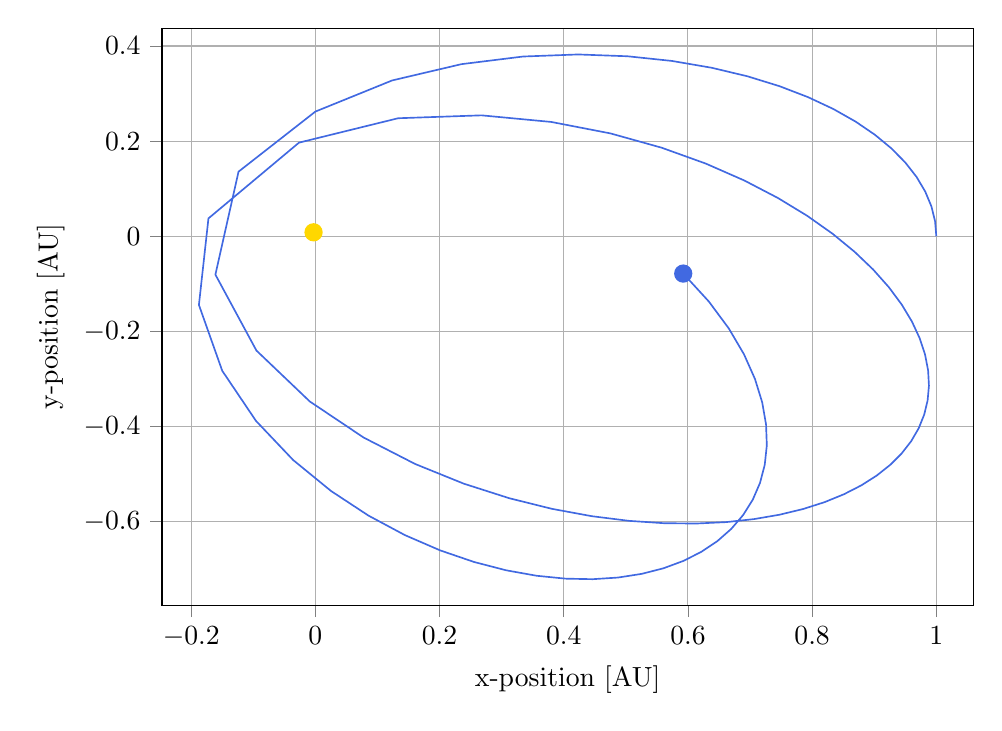
\begin{tikzpicture}

\definecolor{color0}{rgb}{1,0.843137254901961,0}
\definecolor{color1}{rgb}{0.254901960784314,0.411764705882353,0.882352941176471}

\begin{axis}[
height=\figureheight,
tick align=outside,
tick pos=left,
width=\figurewidth,
x grid style={white!69.01960784313725!black},
xlabel={x-position [AU]},
xmajorgrids,
xmin=-0.24694745, xmax=1.05937845,
y grid style={white!69.01960784313725!black},
ylabel={y-position [AU]},
ymajorgrids,
ymin=-0.77644385, ymax=0.43738085
]
\addplot [semithick, color0, forget plot]
table [row sep=\\]{%
-0.00018544	0.00726177 \\
-0.000213167	0.00727106 \\
-0.000240883	0.00728036 \\
-0.000268587	0.00728965 \\
-0.000296278	0.00729895 \\
-0.000323958	0.00730825 \\
-0.000351624	0.00731755 \\
-0.000379278	0.00732685 \\
-0.000406918	0.00733616 \\
-0.000434544	0.00734547 \\
-0.000462155	0.00735478 \\
-0.00048975	0.0073641 \\
-0.000517329	0.00737343 \\
-0.000544889	0.00738276 \\
-0.00057243	0.00739211 \\
-0.000599949	0.00740147 \\
-0.000627444	0.00741085 \\
-0.000654911	0.00742025 \\
-0.000682346	0.00742969 \\
-0.000709744	0.00743918 \\
-0.000737107	0.00744877 \\
-0.000764469	0.00745853 \\
-0.00079209	0.00746857 \\
-0.000820022	0.00747844 \\
-0.000848014	0.00748815 \\
-0.000876008	0.00749777 \\
-0.000903991	0.00750733 \\
-0.000931959	0.00751684 \\
-0.000959913	0.00752632 \\
-0.000987853	0.00753578 \\
-0.00101578	0.00754522 \\
-0.00104369	0.00755463 \\
-0.00107159	0.00756404 \\
-0.00109948	0.00757343 \\
-0.00112736	0.00758281 \\
-0.00115523	0.00759218 \\
-0.00118309	0.00760154 \\
-0.00121094	0.0076109 \\
-0.00123877	0.00762024 \\
-0.0012666	0.00762958 \\
-0.00129442	0.00763892 \\
-0.00132223	0.00764824 \\
-0.00135002	0.00765756 \\
-0.00137781	0.00766688 \\
-0.00140559	0.00767619 \\
-0.00143336	0.0076855 \\
-0.00146112	0.0076948 \\
-0.00148887	0.0077041 \\
-0.00151661	0.0077134 \\
-0.00154434	0.00772269 \\
-0.00157206	0.00773198 \\
-0.00159977	0.00774127 \\
-0.00162747	0.00775055 \\
-0.00165515	0.00775984 \\
-0.00168282	0.00776912 \\
-0.00171048	0.00777839 \\
-0.00173812	0.00778767 \\
-0.00176575	0.00779695 \\
-0.00179336	0.00780622 \\
-0.00182095	0.0078155 \\
-0.00184852	0.00782478 \\
-0.00187607	0.00783406 \\
-0.00190359	0.00784335 \\
-0.00193108	0.00785265 \\
-0.00195852	0.00786197 \\
-0.00198592	0.00787131 \\
-0.00201325	0.00788072 \\
-0.0020405	0.00789026 \\
-0.0020678	0.00790013 \\
-0.00209549	0.00791007 \\
-0.00212333	0.00791987 \\
-0.00215123	0.00792958 \\
-0.00217914	0.00793922 \\
-0.00220706	0.0079488 \\
-0.00223497	0.00795835 \\
-0.00226288	0.00796786 \\
-0.00229079	0.00797734 \\
-0.00231868	0.00798681 \\
-0.00234657	0.00799625 \\
-0.00237445	0.00800567 \\
-0.00240233	0.00801508 \\
-0.00243019	0.00802447 \\
-0.00245805	0.00803385 \\
-0.0024859	0.00804322 \\
-0.00251374	0.00805257 \\
-0.00254157	0.00806192 \\
-0.00256939	0.00807125 \\
-0.0025972	0.00808057 \\
-0.002625	0.00808988 \\
-0.00265279	0.00809918 \\
-0.00268057	0.00810848 \\
-0.00270834	0.00811776 \\
-0.00273609	0.00812703 \\
-0.00276384	0.0081363 \\
-0.00279157	0.00814556 \\
-0.00281928	0.00815481 \\
-0.00284698	0.00816405 \\
-0.00287466	0.00817328 \\
-0.00290232	0.00818251 \\
-0.00292996	0.00819173 \\
-0.00295757	0.00820094 \\
};
\addplot [semithick, color0, mark=*, mark size=3, mark options={solid}, only marks, forget plot]
table [row sep=\\]{%
-0.00295757	0.00820094 \\
};
\addplot [semithick, color1, forget plot]
table [row sep=\\]{%
1	0 \\
0.998027	0.0314303 \\
0.992096	0.0627647 \\
0.982174	0.093876 \\
0.968209	0.124631 \\
0.950127	0.154887 \\
0.927828	0.184489 \\
0.901185	0.213261 \\
0.870043	0.241006 \\
0.834207	0.26749 \\
0.793439	0.292437 \\
0.74745	0.31551 \\
0.695882	0.336284 \\
0.638296	0.354216 \\
0.574144	0.368583 \\
0.502738	0.37839 \\
0.423204	0.382207 \\
0.334431	0.377855 \\
0.235044	0.361768 \\
0.123583	0.327533 \\
3.41517e-06	0.262086 \\
-0.123754	0.135755 \\
-0.161018	-0.0808008 \\
-0.0949526	-0.240432 \\
-0.00895822	-0.347578 \\
0.0777508	-0.423434 \\
0.160767	-0.479051 \\
0.239048	-0.520415 \\
0.31247	-0.551093 \\
0.381185	-0.57338 \\
0.445412	-0.588846 \\
0.505377	-0.598617 \\
0.561284	-0.603532 \\
0.613316	-0.604234 \\
0.661626	-0.601232 \\
0.706347	-0.594932 \\
0.747587	-0.585668 \\
0.785437	-0.573718 \\
0.819968	-0.559315 \\
0.851237	-0.54266 \\
0.879284	-0.523926 \\
0.904136	-0.503263 \\
0.925808	-0.480805 \\
0.944299	-0.456672 \\
0.959598	-0.430971 \\
0.971678	-0.403801 \\
0.980501	-0.375253 \\
0.986013	-0.345415 \\
0.988145	-0.314367 \\
0.986811	-0.282192 \\
0.981907	-0.24897 \\
0.973305	-0.214782 \\
0.960854	-0.179716 \\
0.944373	-0.143865 \\
0.923645	-0.107333 \\
0.898412	-0.0702409 \\
0.868361	-0.0327311 \\
0.833112	0.00502075 \\
0.792199	0.0427915 \\
0.745042	0.080287 \\
0.690906	0.117105 \\
0.628842	0.152673 \\
0.557591	0.186131 \\
0.47543	0.216113 \\
0.37993	0.240274 \\
0.267555	0.254167 \\
0.133319	0.248083 \\
-0.0264107	0.19675 \\
-0.172208	0.0374425 \\
-0.187569	-0.144514 \\
-0.150008	-0.282978 \\
-0.0956482	-0.388397 \\
-0.0358213	-0.470642 \\
0.0252084	-0.535779 \\
0.0855673	-0.587612 \\
0.144337	-0.628669 \\
0.201032	-0.660711 \\
0.255375	-0.685022 \\
0.307202	-0.702563 \\
0.356403	-0.71408 \\
0.402903	-0.720159 \\
0.446638	-0.72127 \\
0.487551	-0.717799 \\
0.525584	-0.710062 \\
0.560673	-0.698321 \\
0.592747	-0.682799 \\
0.621723	-0.66368 \\
0.647502	-0.641123 \\
0.669972	-0.61526 \\
0.688999	-0.586207 \\
0.704425	-0.55406 \\
0.716065	-0.518902 \\
0.723696	-0.480806 \\
0.727056	-0.439834 \\
0.725828	-0.396047 \\
0.719628	-0.3495 \\
0.707983	-0.300259 \\
0.690306	-0.2484 \\
0.665852	-0.194033 \\
0.633657	-0.137326 \\
0.592436	-0.0785546 \\
};
\addplot [semithick, color1, mark=*, mark size=3, mark options={solid}, only marks, forget plot]
table [row sep=\\]{%
0.592436	-0.0785546 \\
};
\end{axis}

\end{tikzpicture}
     \caption{The Earth-Sun system with initial conditions $v = 2 \pi$ AU/year and $r = 1$ AU simulated using velocity Verlet over a period of 1 year with $dt = 0.01$. The yellow dot represents the Sun and the blue represents the Earth. }
     \label{fig:circular}
 \end{figure}
 
The Earth simulated in figure \ref{fig:circular} has an eccentricity of 0. Eccentricity is a measure of how much a planetary orbit deviates from being perfectly circular. In reality, Earth has an eccentricity of 0.0167 \cite{earthfactsheet} which closely represents a perfect circle. The true velocity of Earth is therefore not exactly $v = 2 \pi$ AU/year, but very close. Using NASA's HORIZONS tool, we find that the Earth has an initial velocity of $v = 6.3112$ AU/year.

We can further study the eccentricity and stability of Earths orbit by altering the initial velocity to $v = \pi$ AU/yr. This is then simulated for the two scenarios seen in figure \ref{fig:elliptical_pi}, one with a stepszise of $dt = 0.01$ seen in subfigure (A), and one with $dt = 0.001$ seen in (B), both over a period of 1 year. We see that the velocity is too low to keep Earth in a circular orbit, and the planet accelerates towards the Sun resulting in elliptical orbits. The simulation in (A) has a low precision, and results in an unstable orbit where the perihelion of Earth changes with every orbit. We also see that the orbital period is affected, as Earth completes more that one orbit per year.

The simulation in (B) with better precision results in a more stable elliptical orbit. This suggests that the stepsize should be picked with care, as the outcome of the simulation can be drastically different depending on your choice. As mentioned in section \ref{sec:method}, the error in the velocity Verlet method is proportional to the stepsize cubed, meaning that the simulation in (B) represents a more realistic scenario than the simulation in (A). The orbital period is still altered however as we see the earth continuing past its initial position (denoted as a faint blue marker). 


\begin{figure}
    \centering
    \subfloat[Stepsize $dt = 0.01$]{ \input{figures/elliptical_pi_unstable.tex}}
    \subfloat[Stepsize $dt = 0.001$]{ % This file was created by matplotlib2tikz v0.6.18.
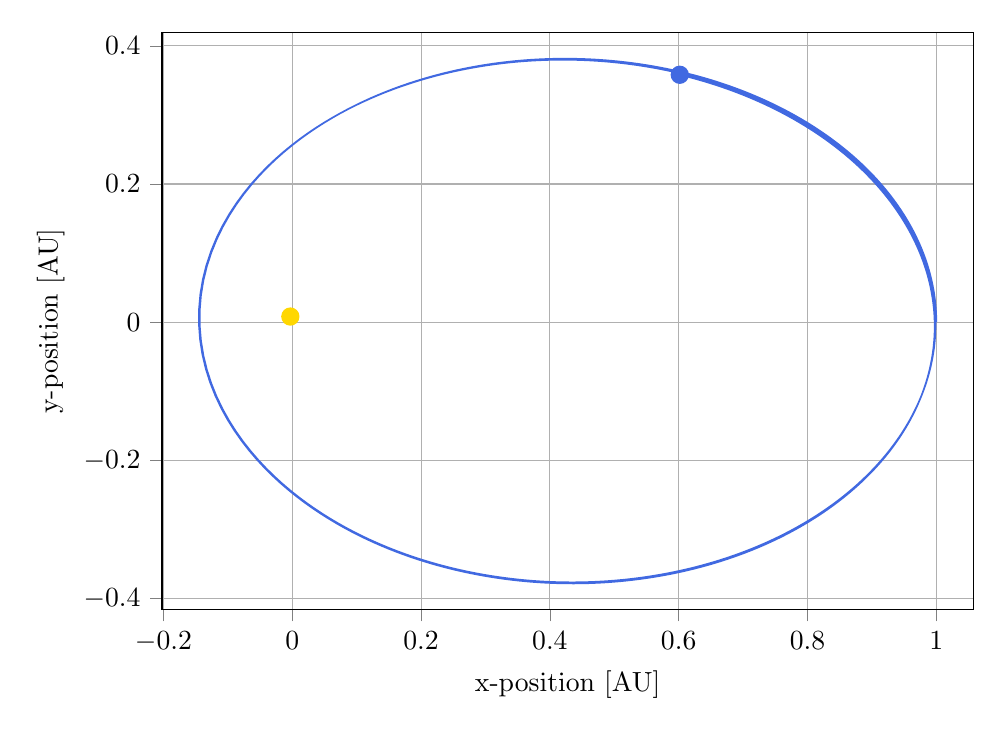
\begin{tikzpicture}

\definecolor{color0}{rgb}{1,0.843137254901961,0}
\definecolor{color1}{rgb}{0.254901960784314,0.411764705882353,0.882352941176471}

\begin{axis}[
height=\figureheight,
tick align=outside,
tick pos=left,
width=\figurewidth,
x grid style={white!69.01960784313725!black},
xlabel={x-position [AU]},
xmajorgrids,
xmin=-0.20215235, xmax=1.05724535,
y grid style={white!69.01960784313725!black},
ylabel={y-position [AU]},
ymajorgrids,
ymin=-0.415978, ymax=0.41934
]
\addplot [semithick, color0, forget plot]
table [row sep=\\]{%
-0.00018544	0.00726177 \\
-0.000188213	0.00726269 \\
-0.000190986	0.00726362 \\
-0.000193759	0.00726455 \\
-0.000196532	0.00726548 \\
-0.000199305	0.00726641 \\
-0.000202078	0.00726734 \\
-0.00020485	0.00726827 \\
-0.000207623	0.0072692 \\
-0.000210395	0.00727013 \\
-0.000213167	0.00727106 \\
-0.00021594	0.00727199 \\
-0.000218712	0.00727292 \\
-0.000221483	0.00727385 \\
-0.000224255	0.00727478 \\
-0.000227027	0.00727571 \\
-0.000229798	0.00727664 \\
-0.00023257	0.00727757 \\
-0.000235341	0.0072785 \\
-0.000238112	0.00727943 \\
-0.000240883	0.00728036 \\
-0.000243654	0.00728129 \\
-0.000246425	0.00728221 \\
-0.000249196	0.00728314 \\
-0.000251966	0.00728407 \\
-0.000254736	0.007285 \\
-0.000257507	0.00728593 \\
-0.000260277	0.00728686 \\
-0.000263047	0.00728779 \\
-0.000265817	0.00728872 \\
-0.000268587	0.00728965 \\
-0.000271357	0.00729058 \\
-0.000274126	0.00729151 \\
-0.000276896	0.00729244 \\
-0.000279665	0.00729337 \\
-0.000282434	0.0072943 \\
-0.000285203	0.00729523 \\
-0.000287972	0.00729616 \\
-0.000290741	0.00729709 \\
-0.00029351	0.00729802 \\
-0.000296278	0.00729895 \\
-0.000299047	0.00729988 \\
-0.000301815	0.00730081 \\
-0.000304583	0.00730174 \\
-0.000307352	0.00730267 \\
-0.00031012	0.0073036 \\
-0.000312887	0.00730453 \\
-0.000315655	0.00730546 \\
-0.000318423	0.00730639 \\
-0.00032119	0.00730732 \\
-0.000323958	0.00730825 \\
-0.000326725	0.00730918 \\
-0.000329492	0.00731011 \\
-0.000332259	0.00731104 \\
-0.000335026	0.00731197 \\
-0.000337792	0.0073129 \\
-0.000340559	0.00731383 \\
-0.000343325	0.00731476 \\
-0.000346092	0.00731569 \\
-0.000348858	0.00731662 \\
-0.000351624	0.00731755 \\
-0.00035439	0.00731848 \\
-0.000357156	0.00731941 \\
-0.000359922	0.00732034 \\
-0.000362687	0.00732127 \\
-0.000365452	0.0073222 \\
-0.000368218	0.00732313 \\
-0.000370983	0.00732406 \\
-0.000373748	0.00732499 \\
-0.000376513	0.00732592 \\
-0.000379278	0.00732685 \\
-0.000382042	0.00732778 \\
-0.000384807	0.00732871 \\
-0.000387571	0.00732964 \\
-0.000390335	0.00733057 \\
-0.000393099	0.0073315 \\
-0.000395863	0.00733243 \\
-0.000398627	0.00733336 \\
-0.000401391	0.0073343 \\
-0.000404154	0.00733523 \\
-0.000406917	0.00733616 \\
-0.000409681	0.00733709 \\
-0.000412444	0.00733802 \\
-0.000415207	0.00733895 \\
-0.00041797	0.00733988 \\
-0.000420732	0.00734081 \\
-0.000423495	0.00734174 \\
-0.000426257	0.00734267 \\
-0.000429019	0.0073436 \\
-0.000431781	0.00734454 \\
-0.000434543	0.00734547 \\
-0.000437305	0.0073464 \\
-0.000440067	0.00734733 \\
-0.000442828	0.00734826 \\
-0.000445589	0.00734919 \\
-0.000448351	0.00735012 \\
-0.000451112	0.00735106 \\
-0.000453873	0.00735199 \\
-0.000456633	0.00735292 \\
-0.000459394	0.00735385 \\
-0.000462154	0.00735478 \\
-0.000464915	0.00735571 \\
-0.000467675	0.00735665 \\
-0.000470435	0.00735758 \\
-0.000473194	0.00735851 \\
-0.000475954	0.00735944 \\
-0.000478713	0.00736037 \\
-0.000481473	0.00736131 \\
-0.000484232	0.00736224 \\
-0.000486991	0.00736317 \\
-0.00048975	0.0073641 \\
-0.000492508	0.00736503 \\
-0.000495267	0.00736597 \\
-0.000498025	0.0073669 \\
-0.000500783	0.00736783 \\
-0.000503541	0.00736876 \\
-0.000506299	0.0073697 \\
-0.000509056	0.00737063 \\
-0.000511814	0.00737156 \\
-0.000514571	0.0073725 \\
-0.000517328	0.00737343 \\
-0.000520085	0.00737436 \\
-0.000522842	0.0073753 \\
-0.000525598	0.00737623 \\
-0.000528354	0.00737716 \\
-0.000531111	0.0073781 \\
-0.000533867	0.00737903 \\
-0.000536622	0.00737996 \\
-0.000539378	0.0073809 \\
-0.000542133	0.00738183 \\
-0.000544888	0.00738276 \\
-0.000547643	0.0073837 \\
-0.000550398	0.00738463 \\
-0.000553153	0.00738557 \\
-0.000555907	0.0073865 \\
-0.000558661	0.00738744 \\
-0.000561415	0.00738837 \\
-0.000564169	0.00738931 \\
-0.000566923	0.00739024 \\
-0.000569676	0.00739118 \\
-0.000572429	0.00739211 \\
-0.000575182	0.00739305 \\
-0.000577935	0.00739398 \\
-0.000580687	0.00739492 \\
-0.000583439	0.00739585 \\
-0.000586191	0.00739679 \\
-0.000588943	0.00739773 \\
-0.000591694	0.00739866 \\
-0.000594446	0.0073996 \\
-0.000597197	0.00740053 \\
-0.000599948	0.00740147 \\
-0.000602698	0.00740241 \\
-0.000605449	0.00740335 \\
-0.000608199	0.00740428 \\
-0.000610948	0.00740522 \\
-0.000613698	0.00740616 \\
-0.000616447	0.0074071 \\
-0.000619196	0.00740803 \\
-0.000621945	0.00740897 \\
-0.000624694	0.00740991 \\
-0.000627442	0.00741085 \\
-0.00063019	0.00741179 \\
-0.000632937	0.00741273 \\
-0.000635685	0.00741367 \\
-0.000638432	0.00741461 \\
-0.000641179	0.00741555 \\
-0.000643925	0.00741649 \\
-0.000646671	0.00741743 \\
-0.000649417	0.00741837 \\
-0.000652163	0.00741931 \\
-0.000654908	0.00742025 \\
-0.000657653	0.0074212 \\
-0.000660398	0.00742214 \\
-0.000663142	0.00742308 \\
-0.000665886	0.00742402 \\
-0.000668629	0.00742497 \\
-0.000671373	0.00742591 \\
-0.000674116	0.00742686 \\
-0.000676858	0.0074278 \\
-0.0006796	0.00742875 \\
-0.000682342	0.00742969 \\
-0.000685084	0.00743064 \\
-0.000687825	0.00743159 \\
-0.000690565	0.00743253 \\
-0.000693306	0.00743348 \\
-0.000696046	0.00743443 \\
-0.000698785	0.00743538 \\
-0.000701525	0.00743633 \\
-0.000704263	0.00743728 \\
-0.000707002	0.00743824 \\
-0.00070974	0.00743919 \\
-0.000712478	0.00744014 \\
-0.000715215	0.0074411 \\
-0.000717952	0.00744206 \\
-0.000720689	0.00744301 \\
-0.000723425	0.00744397 \\
-0.000726161	0.00744493 \\
-0.000728897	0.00744589 \\
-0.000731632	0.00744686 \\
-0.000734368	0.00744782 \\
-0.000737103	0.00744879 \\
-0.000739838	0.00744975 \\
-0.000742574	0.00745072 \\
-0.00074531	0.0074517 \\
-0.000748046	0.00745267 \\
-0.000750783	0.00745365 \\
-0.00075352	0.00745463 \\
-0.000756259	0.00745561 \\
-0.000759	0.0074566 \\
-0.000761742	0.00745759 \\
-0.000764488	0.00745858 \\
-0.000767236	0.00745958 \\
-0.000769989	0.00746058 \\
-0.000772746	0.00746158 \\
-0.000775508	0.00746258 \\
-0.000778276	0.00746359 \\
-0.000781049	0.00746459 \\
-0.000783828	0.0074656 \\
-0.000786613	0.0074666 \\
-0.000789403	0.0074676 \\
-0.000792197	0.0074686 \\
-0.000794995	0.00746959 \\
-0.000797796	0.00747059 \\
-0.000800599	0.00747158 \\
-0.000803405	0.00747256 \\
-0.000806212	0.00747355 \\
-0.00080902	0.00747453 \\
-0.000811829	0.0074755 \\
-0.000814639	0.00747648 \\
-0.00081745	0.00747745 \\
-0.00082026	0.00747842 \\
-0.000823071	0.00747939 \\
-0.000825882	0.00748036 \\
-0.000828692	0.00748132 \\
-0.000831503	0.00748229 \\
-0.000834313	0.00748325 \\
-0.000837123	0.00748421 \\
-0.000839933	0.00748517 \\
-0.000842742	0.00748613 \\
-0.000845552	0.00748708 \\
-0.00084836	0.00748804 \\
-0.000851169	0.00748899 \\
-0.000853977	0.00748995 \\
-0.000856785	0.0074909 \\
-0.000859592	0.00749185 \\
-0.000862399	0.0074928 \\
-0.000865206	0.00749375 \\
-0.000868013	0.0074947 \\
-0.000870819	0.00749565 \\
-0.000873624	0.0074966 \\
-0.000876429	0.00749755 \\
-0.000879234	0.00749849 \\
-0.000882039	0.00749944 \\
-0.000884843	0.00750039 \\
-0.000887647	0.00750133 \\
-0.000890451	0.00750228 \\
-0.000893254	0.00750322 \\
-0.000896057	0.00750417 \\
-0.000898859	0.00750511 \\
-0.000901661	0.00750605 \\
-0.000904463	0.007507 \\
-0.000907265	0.00750794 \\
-0.000910066	0.00750888 \\
-0.000912867	0.00750982 \\
-0.000915668	0.00751077 \\
-0.000918468	0.00751171 \\
-0.000921268	0.00751265 \\
-0.000924068	0.00751359 \\
-0.000926867	0.00751453 \\
-0.000929667	0.00751547 \\
-0.000932466	0.00751641 \\
-0.000935264	0.00751735 \\
-0.000938063	0.00751829 \\
-0.000940861	0.00751923 \\
-0.000943659	0.00752017 \\
-0.000946456	0.0075211 \\
-0.000949253	0.00752204 \\
-0.00095205	0.00752298 \\
-0.000954847	0.00752392 \\
-0.000957644	0.00752486 \\
-0.00096044	0.00752579 \\
-0.000963236	0.00752673 \\
-0.000966032	0.00752767 \\
-0.000968828	0.00752861 \\
-0.000971623	0.00752954 \\
-0.000974418	0.00753048 \\
-0.000977213	0.00753142 \\
-0.000980008	0.00753235 \\
-0.000982802	0.00753329 \\
-0.000985597	0.00753422 \\
-0.000988391	0.00753516 \\
-0.000991184	0.0075361 \\
-0.000993978	0.00753703 \\
-0.000996771	0.00753797 \\
-0.000999564	0.0075389 \\
-0.00100236	0.00753984 \\
-0.00100515	0.00754077 \\
-0.00100794	0.00754171 \\
-0.00101074	0.00754264 \\
-0.00101353	0.00754358 \\
-0.00101632	0.00754451 \\
-0.00101911	0.00754545 \\
-0.0010219	0.00754638 \\
-0.00102469	0.00754732 \\
-0.00102749	0.00754825 \\
-0.00103028	0.00754918 \\
-0.00103307	0.00755012 \\
-0.00103586	0.00755105 \\
-0.00103865	0.00755199 \\
-0.00104144	0.00755292 \\
-0.00104423	0.00755385 \\
-0.00104702	0.00755479 \\
-0.00104981	0.00755572 \\
-0.0010526	0.00755665 \\
-0.00105539	0.00755759 \\
-0.00105818	0.00755852 \\
-0.00106096	0.00755945 \\
-0.00106375	0.00756039 \\
-0.00106654	0.00756132 \\
-0.00106933	0.00756225 \\
-0.00107212	0.00756318 \\
-0.00107491	0.00756412 \\
-0.0010777	0.00756505 \\
-0.00108048	0.00756598 \\
-0.00108327	0.00756691 \\
-0.00108606	0.00756785 \\
-0.00108885	0.00756878 \\
-0.00109163	0.00756971 \\
-0.00109442	0.00757064 \\
-0.00109721	0.00757158 \\
-0.00109999	0.00757251 \\
-0.00110278	0.00757344 \\
-0.00110557	0.00757437 \\
-0.00110835	0.0075753 \\
-0.00111114	0.00757624 \\
-0.00111392	0.00757717 \\
-0.00111671	0.0075781 \\
-0.0011195	0.00757903 \\
-0.00112228	0.00757996 \\
-0.00112507	0.00758089 \\
-0.00112785	0.00758183 \\
-0.00113064	0.00758276 \\
-0.00113342	0.00758369 \\
-0.00113621	0.00758462 \\
-0.00113899	0.00758555 \\
-0.00114178	0.00758648 \\
-0.00114456	0.00758741 \\
-0.00114734	0.00758835 \\
-0.00115013	0.00758928 \\
-0.00115291	0.00759021 \\
-0.0011557	0.00759114 \\
-0.00115848	0.00759207 \\
-0.00116126	0.007593 \\
-0.00116405	0.00759393 \\
-0.00116683	0.00759486 \\
-0.00116961	0.00759579 \\
-0.0011724	0.00759672 \\
-0.00117518	0.00759766 \\
-0.00117796	0.00759859 \\
-0.00118074	0.00759952 \\
-0.00118353	0.00760045 \\
-0.00118631	0.00760138 \\
-0.00118909	0.00760231 \\
-0.00119187	0.00760324 \\
-0.00119465	0.00760417 \\
-0.00119744	0.0076051 \\
-0.00120022	0.00760603 \\
-0.001203	0.00760696 \\
-0.00120578	0.00760789 \\
-0.00120856	0.00760882 \\
-0.00121134	0.00760975 \\
-0.00121412	0.00761068 \\
-0.0012169	0.00761161 \\
-0.00121968	0.00761254 \\
-0.00122246	0.00761347 \\
-0.00122525	0.0076144 \\
-0.00122803	0.00761533 \\
-0.00123081	0.00761626 \\
-0.00123359	0.00761719 \\
-0.00123637	0.00761813 \\
-0.00123915	0.00761906 \\
-0.00124193	0.00761999 \\
-0.0012447	0.00762092 \\
-0.00124748	0.00762185 \\
-0.00125026	0.00762278 \\
-0.00125304	0.00762371 \\
-0.00125582	0.00762464 \\
-0.0012586	0.00762557 \\
-0.00126138	0.0076265 \\
-0.00126416	0.00762743 \\
-0.00126694	0.00762836 \\
-0.00126971	0.00762929 \\
-0.00127249	0.00763021 \\
-0.00127527	0.00763114 \\
-0.00127805	0.00763207 \\
-0.00128083	0.007633 \\
-0.0012836	0.00763393 \\
-0.00128638	0.00763486 \\
-0.00128916	0.00763579 \\
-0.00129194	0.00763672 \\
-0.00129471	0.00763765 \\
-0.00129749	0.00763858 \\
-0.00130027	0.00763951 \\
-0.00130305	0.00764044 \\
-0.00130582	0.00764137 \\
-0.0013086	0.0076423 \\
-0.00131138	0.00764323 \\
-0.00131415	0.00764416 \\
-0.00131693	0.00764509 \\
-0.0013197	0.00764602 \\
-0.00132248	0.00764695 \\
-0.00132526	0.00764788 \\
-0.00132803	0.00764881 \\
-0.00133081	0.00764974 \\
-0.00133358	0.00765067 \\
-0.00133636	0.0076516 \\
-0.00133913	0.00765253 \\
-0.00134191	0.00765346 \\
-0.00134468	0.00765439 \\
-0.00134746	0.00765532 \\
-0.00135023	0.00765625 \\
-0.00135301	0.00765718 \\
-0.00135578	0.00765811 \\
-0.00135856	0.00765903 \\
-0.00136133	0.00765996 \\
-0.00136411	0.00766089 \\
-0.00136688	0.00766182 \\
-0.00136966	0.00766275 \\
-0.00137243	0.00766368 \\
-0.0013752	0.00766461 \\
-0.00137798	0.00766554 \\
-0.00138075	0.00766647 \\
-0.00138352	0.0076674 \\
-0.0013863	0.00766833 \\
-0.00138907	0.00766926 \\
-0.00139184	0.00767019 \\
-0.00139462	0.00767112 \\
-0.00139739	0.00767205 \\
-0.00140016	0.00767298 \\
-0.00140293	0.00767391 \\
-0.00140571	0.00767484 \\
-0.00140848	0.00767577 \\
-0.00141125	0.0076767 \\
-0.00141402	0.00767762 \\
-0.0014168	0.00767855 \\
-0.00141957	0.00767948 \\
-0.00142234	0.00768041 \\
-0.00142511	0.00768134 \\
-0.00142788	0.00768227 \\
-0.00143065	0.0076832 \\
-0.00143343	0.00768413 \\
-0.0014362	0.00768506 \\
-0.00143897	0.00768599 \\
-0.00144174	0.00768692 \\
-0.00144451	0.00768785 \\
-0.00144728	0.00768878 \\
-0.00145005	0.00768971 \\
-0.00145282	0.00769064 \\
-0.00145559	0.00769157 \\
-0.00145836	0.0076925 \\
-0.00146113	0.00769343 \\
-0.0014639	0.00769436 \\
-0.00146667	0.00769529 \\
-0.00146944	0.00769622 \\
-0.00147221	0.00769715 \\
-0.00147498	0.00769808 \\
-0.00147775	0.00769901 \\
-0.00148052	0.00769993 \\
-0.00148329	0.00770086 \\
-0.00148606	0.00770179 \\
-0.00148883	0.00770272 \\
-0.0014916	0.00770365 \\
-0.00149436	0.00770458 \\
-0.00149713	0.00770551 \\
-0.0014999	0.00770644 \\
-0.00150267	0.00770737 \\
-0.00150544	0.0077083 \\
-0.00150821	0.00770923 \\
-0.00151097	0.00771016 \\
-0.00151374	0.00771109 \\
-0.00151651	0.00771202 \\
-0.00151928	0.00771295 \\
-0.00152204	0.00771388 \\
-0.00152481	0.00771481 \\
-0.00152758	0.00771574 \\
-0.00153035	0.00771667 \\
-0.00153311	0.0077176 \\
-0.00153588	0.00771853 \\
-0.00153865	0.00771946 \\
-0.00154141	0.00772039 \\
-0.00154418	0.00772132 \\
-0.00154694	0.00772225 \\
-0.00154971	0.00772318 \\
-0.00155248	0.00772411 \\
-0.00155524	0.00772504 \\
-0.00155801	0.00772597 \\
-0.00156077	0.0077269 \\
-0.00156354	0.00772783 \\
-0.00156631	0.00772876 \\
-0.00156907	0.00772969 \\
-0.00157184	0.00773062 \\
-0.0015746	0.00773155 \\
-0.00157737	0.00773248 \\
-0.00158013	0.00773342 \\
-0.00158289	0.00773435 \\
-0.00158566	0.00773528 \\
-0.00158842	0.00773621 \\
-0.00159119	0.00773714 \\
-0.00159395	0.00773807 \\
-0.00159671	0.007739 \\
-0.00159948	0.00773993 \\
-0.00160224	0.00774086 \\
-0.00160501	0.00774179 \\
-0.00160777	0.00774272 \\
-0.00161053	0.00774365 \\
-0.00161329	0.00774458 \\
-0.00161606	0.00774551 \\
-0.00161882	0.00774644 \\
-0.00162158	0.00774738 \\
-0.00162435	0.00774831 \\
-0.00162711	0.00774924 \\
-0.00162987	0.00775017 \\
-0.00163263	0.0077511 \\
-0.00163539	0.00775203 \\
-0.00163816	0.00775296 \\
-0.00164092	0.00775389 \\
-0.00164368	0.00775482 \\
-0.00164644	0.00775576 \\
-0.0016492	0.00775669 \\
-0.00165196	0.00775762 \\
-0.00165472	0.00775855 \\
-0.00165748	0.00775948 \\
-0.00166024	0.00776041 \\
-0.001663	0.00776135 \\
-0.00166576	0.00776228 \\
-0.00166852	0.00776321 \\
-0.00167128	0.00776414 \\
-0.00167404	0.00776507 \\
-0.0016768	0.007766 \\
-0.00167956	0.00776694 \\
-0.00168232	0.00776787 \\
-0.00168508	0.0077688 \\
-0.00168784	0.00776973 \\
-0.0016906	0.00777067 \\
-0.00169336	0.0077716 \\
-0.00169611	0.00777253 \\
-0.00169887	0.00777346 \\
-0.00170163	0.0077744 \\
-0.00170439	0.00777533 \\
-0.00170715	0.00777626 \\
-0.0017099	0.00777719 \\
-0.00171266	0.00777813 \\
-0.00171542	0.00777906 \\
-0.00171817	0.00777999 \\
-0.00172093	0.00778093 \\
-0.00172369	0.00778186 \\
-0.00172644	0.00778279 \\
-0.0017292	0.00778373 \\
-0.00173196	0.00778466 \\
-0.00173471	0.00778559 \\
-0.00173747	0.00778653 \\
-0.00174022	0.00778746 \\
-0.00174298	0.00778839 \\
-0.00174573	0.00778933 \\
-0.00174849	0.00779026 \\
-0.00175124	0.0077912 \\
-0.001754	0.00779213 \\
-0.00175675	0.00779307 \\
-0.00175951	0.007794 \\
-0.00176226	0.00779494 \\
-0.00176501	0.00779587 \\
-0.00176777	0.00779681 \\
-0.00177052	0.00779774 \\
-0.00177327	0.00779868 \\
-0.00177602	0.00779961 \\
-0.00177878	0.00780055 \\
-0.00178153	0.00780148 \\
-0.00178428	0.00780242 \\
-0.00178703	0.00780335 \\
-0.00178978	0.00780429 \\
-0.00179254	0.00780523 \\
-0.00179529	0.00780616 \\
-0.00179804	0.0078071 \\
-0.00180079	0.00780804 \\
-0.00180354	0.00780897 \\
-0.00180629	0.00780991 \\
-0.00180904	0.00781085 \\
-0.00181179	0.00781179 \\
-0.00181454	0.00781272 \\
-0.00181729	0.00781366 \\
-0.00182004	0.0078146 \\
-0.00182278	0.00781554 \\
-0.00182553	0.00781648 \\
-0.00182828	0.00781742 \\
-0.00183103	0.00781836 \\
-0.00183378	0.00781929 \\
-0.00183652	0.00782023 \\
-0.00183927	0.00782117 \\
-0.00184202	0.00782211 \\
-0.00184476	0.00782306 \\
-0.00184751	0.007824 \\
-0.00185025	0.00782494 \\
-0.001853	0.00782588 \\
-0.00185574	0.00782682 \\
-0.00185849	0.00782776 \\
-0.00186123	0.00782871 \\
-0.00186398	0.00782965 \\
-0.00186672	0.00783059 \\
-0.00186946	0.00783154 \\
-0.00187221	0.00783248 \\
-0.00187495	0.00783343 \\
-0.00187769	0.00783437 \\
-0.00188043	0.00783532 \\
-0.00188317	0.00783626 \\
-0.00188592	0.00783721 \\
-0.00188866	0.00783816 \\
-0.0018914	0.00783911 \\
-0.00189414	0.00784006 \\
-0.00189688	0.00784101 \\
-0.00189962	0.00784196 \\
-0.00190235	0.00784291 \\
-0.00190509	0.00784386 \\
-0.00190783	0.00784481 \\
-0.00191057	0.00784577 \\
-0.00191331	0.00784672 \\
-0.00191604	0.00784768 \\
-0.00191878	0.00784863 \\
-0.00192151	0.00784959 \\
-0.00192425	0.00785055 \\
-0.00192699	0.00785151 \\
-0.00192972	0.00785248 \\
-0.00193246	0.00785344 \\
-0.00193519	0.00785441 \\
-0.00193793	0.00785537 \\
-0.00194066	0.00785634 \\
-0.0019434	0.00785732 \\
-0.00194613	0.00785829 \\
-0.00194887	0.00785927 \\
-0.00195161	0.00786025 \\
-0.00195435	0.00786123 \\
-0.00195709	0.00786222 \\
-0.00195983	0.00786321 \\
-0.00196257	0.0078642 \\
-0.00196532	0.0078652 \\
-0.00196807	0.00786619 \\
-0.00197083	0.0078672 \\
-0.00197359	0.0078682 \\
-0.00197636	0.0078692 \\
-0.00197913	0.00787021 \\
-0.00198191	0.00787121 \\
-0.0019847	0.00787222 \\
-0.00198749	0.00787322 \\
-0.00199028	0.00787422 \\
-0.00199308	0.00787521 \\
-0.00199588	0.0078762 \\
-0.00199868	0.00787719 \\
-0.00200149	0.00787818 \\
-0.00200429	0.00787916 \\
-0.0020071	0.00788015 \\
-0.00200991	0.00788112 \\
-0.00201272	0.0078821 \\
-0.00201553	0.00788307 \\
-0.00201834	0.00788404 \\
-0.00202115	0.00788501 \\
-0.00202396	0.00788598 \\
-0.00202677	0.00788694 \\
-0.00202958	0.00788791 \\
-0.00203239	0.00788887 \\
-0.0020352	0.00788983 \\
-0.00203801	0.00789079 \\
-0.00204082	0.00789175 \\
-0.00204363	0.0078927 \\
-0.00204644	0.00789366 \\
-0.00204925	0.00789461 \\
-0.00205206	0.00789557 \\
-0.00205486	0.00789652 \\
-0.00205767	0.00789747 \\
-0.00206048	0.00789842 \\
-0.00206328	0.00789938 \\
-0.00206609	0.00790033 \\
-0.0020689	0.00790127 \\
-0.0020717	0.00790222 \\
-0.00207451	0.00790317 \\
-0.00207731	0.00790412 \\
-0.00208012	0.00790506 \\
-0.00208292	0.00790601 \\
-0.00208572	0.00790696 \\
-0.00208853	0.0079079 \\
-0.00209133	0.00790885 \\
-0.00209413	0.00790979 \\
-0.00209694	0.00791074 \\
-0.00209974	0.00791168 \\
-0.00210254	0.00791262 \\
-0.00210534	0.00791356 \\
-0.00210814	0.00791451 \\
-0.00211094	0.00791545 \\
-0.00211375	0.00791639 \\
-0.00211655	0.00791733 \\
-0.00211935	0.00791827 \\
-0.00212215	0.00791921 \\
-0.00212495	0.00792016 \\
-0.00212774	0.0079211 \\
-0.00213054	0.00792204 \\
-0.00213334	0.00792298 \\
-0.00213614	0.00792391 \\
-0.00213894	0.00792485 \\
-0.00214174	0.00792579 \\
-0.00214453	0.00792673 \\
-0.00214733	0.00792767 \\
-0.00215013	0.00792861 \\
-0.00215293	0.00792955 \\
-0.00215572	0.00793048 \\
-0.00215852	0.00793142 \\
-0.00216131	0.00793236 \\
-0.00216411	0.0079333 \\
-0.00216691	0.00793423 \\
-0.0021697	0.00793517 \\
-0.0021725	0.00793611 \\
-0.00217529	0.00793704 \\
-0.00217809	0.00793798 \\
-0.00218088	0.00793892 \\
-0.00218367	0.00793985 \\
-0.00218647	0.00794079 \\
-0.00218926	0.00794173 \\
-0.00219206	0.00794266 \\
-0.00219485	0.0079436 \\
-0.00219764	0.00794453 \\
-0.00220044	0.00794547 \\
-0.00220323	0.0079464 \\
-0.00220602	0.00794734 \\
-0.00220881	0.00794827 \\
-0.00221161	0.00794921 \\
-0.0022144	0.00795014 \\
-0.00221719	0.00795108 \\
-0.00221998	0.00795201 \\
-0.00222277	0.00795295 \\
-0.00222556	0.00795388 \\
-0.00222835	0.00795481 \\
-0.00223115	0.00795575 \\
-0.00223394	0.00795668 \\
-0.00223673	0.00795762 \\
-0.00223952	0.00795855 \\
-0.00224231	0.00795948 \\
-0.0022451	0.00796042 \\
-0.00224789	0.00796135 \\
-0.00225068	0.00796228 \\
-0.00225347	0.00796322 \\
-0.00225625	0.00796415 \\
-0.00225904	0.00796508 \\
-0.00226183	0.00796602 \\
-0.00226462	0.00796695 \\
-0.00226741	0.00796788 \\
-0.0022702	0.00796882 \\
-0.00227299	0.00796975 \\
-0.00227577	0.00797068 \\
-0.00227856	0.00797161 \\
-0.00228135	0.00797255 \\
-0.00228414	0.00797348 \\
-0.00228693	0.00797441 \\
-0.00228971	0.00797534 \\
-0.0022925	0.00797628 \\
-0.00229529	0.00797721 \\
-0.00229807	0.00797814 \\
-0.00230086	0.00797907 \\
-0.00230365	0.00798 \\
-0.00230643	0.00798094 \\
-0.00230922	0.00798187 \\
-0.002312	0.0079828 \\
-0.00231479	0.00798373 \\
-0.00231758	0.00798466 \\
-0.00232036	0.0079856 \\
-0.00232315	0.00798653 \\
-0.00232593	0.00798746 \\
-0.00232872	0.00798839 \\
-0.0023315	0.00798932 \\
-0.00233429	0.00799025 \\
-0.00233707	0.00799118 \\
-0.00233986	0.00799212 \\
-0.00234264	0.00799305 \\
-0.00234542	0.00799398 \\
-0.00234821	0.00799491 \\
-0.00235099	0.00799584 \\
-0.00235378	0.00799677 \\
-0.00235656	0.0079977 \\
-0.00235934	0.00799863 \\
-0.00236213	0.00799957 \\
-0.00236491	0.0080005 \\
-0.00236769	0.00800143 \\
-0.00237048	0.00800236 \\
-0.00237326	0.00800329 \\
-0.00237604	0.00800422 \\
-0.00237882	0.00800515 \\
-0.00238161	0.00800608 \\
-0.00238439	0.00800701 \\
-0.00238717	0.00800794 \\
-0.00238995	0.00800887 \\
-0.00239273	0.0080098 \\
-0.00239552	0.00801073 \\
-0.0023983	0.00801167 \\
-0.00240108	0.0080126 \\
-0.00240386	0.00801353 \\
-0.00240664	0.00801446 \\
-0.00240942	0.00801539 \\
-0.0024122	0.00801632 \\
-0.00241499	0.00801725 \\
-0.00241777	0.00801818 \\
-0.00242055	0.00801911 \\
-0.00242333	0.00802004 \\
-0.00242611	0.00802097 \\
-0.00242889	0.0080219 \\
-0.00243167	0.00802283 \\
-0.00243445	0.00802376 \\
-0.00243723	0.00802469 \\
-0.00244001	0.00802562 \\
-0.00244279	0.00802655 \\
-0.00244557	0.00802748 \\
-0.00244835	0.00802841 \\
-0.00245112	0.00802934 \\
-0.0024539	0.00803027 \\
-0.00245668	0.0080312 \\
-0.00245946	0.00803213 \\
-0.00246224	0.00803306 \\
-0.00246502	0.00803399 \\
-0.0024678	0.00803492 \\
-0.00247057	0.00803585 \\
-0.00247335	0.00803678 \\
-0.00247613	0.00803771 \\
-0.00247891	0.00803864 \\
-0.00248169	0.00803957 \\
-0.00248446	0.0080405 \\
-0.00248724	0.00804143 \\
-0.00249002	0.00804236 \\
-0.0024928	0.00804329 \\
-0.00249557	0.00804422 \\
-0.00249835	0.00804515 \\
-0.00250113	0.00804608 \\
-0.00250391	0.00804701 \\
-0.00250668	0.00804794 \\
-0.00250946	0.00804887 \\
-0.00251223	0.0080498 \\
-0.00251501	0.00805073 \\
-0.00251779	0.00805166 \\
-0.00252056	0.00805259 \\
-0.00252334	0.00805351 \\
-0.00252612	0.00805444 \\
-0.00252889	0.00805537 \\
-0.00253167	0.0080563 \\
-0.00253444	0.00805723 \\
-0.00253722	0.00805816 \\
-0.00253999	0.00805909 \\
-0.00254277	0.00806002 \\
-0.00254554	0.00806095 \\
-0.00254832	0.00806188 \\
-0.00255109	0.00806281 \\
-0.00255387	0.00806374 \\
-0.00255664	0.00806467 \\
-0.00255942	0.0080656 \\
-0.00256219	0.00806653 \\
-0.00256497	0.00806746 \\
-0.00256774	0.00806839 \\
-0.00257051	0.00806932 \\
-0.00257329	0.00807025 \\
-0.00257606	0.00807118 \\
-0.00257883	0.00807211 \\
-0.00258161	0.00807304 \\
-0.00258438	0.00807397 \\
-0.00258715	0.00807489 \\
-0.00258993	0.00807582 \\
-0.0025927	0.00807675 \\
-0.00259547	0.00807768 \\
-0.00259825	0.00807861 \\
-0.00260102	0.00807954 \\
-0.00260379	0.00808047 \\
-0.00260656	0.0080814 \\
-0.00260934	0.00808233 \\
-0.00261211	0.00808326 \\
-0.00261488	0.00808419 \\
-0.00261765	0.00808512 \\
-0.00262042	0.00808605 \\
-0.0026232	0.00808698 \\
-0.00262597	0.00808791 \\
-0.00262874	0.00808884 \\
-0.00263151	0.00808977 \\
-0.00263428	0.0080907 \\
-0.00263705	0.00809163 \\
-0.00263982	0.00809256 \\
-0.0026426	0.00809348 \\
-0.00264537	0.00809441 \\
-0.00264814	0.00809534 \\
-0.00265091	0.00809627 \\
-0.00265368	0.0080972 \\
-0.00265645	0.00809813 \\
-0.00265922	0.00809906 \\
-0.00266199	0.00809999 \\
-0.00266476	0.00810092 \\
-0.00266753	0.00810185 \\
-0.0026703	0.00810278 \\
-0.00267307	0.00810371 \\
-0.00267584	0.00810464 \\
-0.00267861	0.00810557 \\
-0.00268137	0.0081065 \\
-0.00268414	0.00810743 \\
-0.00268691	0.00810836 \\
-0.00268968	0.00810929 \\
-0.00269245	0.00811022 \\
-0.00269522	0.00811115 \\
-0.00269799	0.00811208 \\
-0.00270076	0.00811301 \\
-0.00270352	0.00811394 \\
-0.00270629	0.00811487 \\
-0.00270906	0.0081158 \\
-0.00271183	0.00811673 \\
-0.0027146	0.00811766 \\
-0.00271736	0.00811859 \\
-0.00272013	0.00811952 \\
-0.0027229	0.00812045 \\
-0.00272567	0.00812138 \\
-0.00272843	0.00812231 \\
-0.0027312	0.00812324 \\
-0.00273397	0.00812417 \\
-0.00273673	0.0081251 \\
-0.0027395	0.00812603 \\
-0.00274227	0.00812696 \\
-0.00274503	0.00812789 \\
-0.0027478	0.00812882 \\
-0.00275056	0.00812975 \\
-0.00275333	0.00813068 \\
-0.0027561	0.00813161 \\
-0.00275886	0.00813254 \\
-0.00276163	0.00813347 \\
-0.00276439	0.0081344 \\
-0.00276716	0.00813533 \\
-0.00276992	0.00813626 \\
-0.00277269	0.00813719 \\
-0.00277545	0.00813812 \\
-0.00277822	0.00813905 \\
-0.00278098	0.00813998 \\
-0.00278375	0.00814091 \\
-0.00278651	0.00814184 \\
-0.00278927	0.00814277 \\
-0.00279204	0.0081437 \\
-0.0027948	0.00814463 \\
-0.00279757	0.00814556 \\
-0.00280033	0.00814649 \\
-0.00280309	0.00814742 \\
-0.00280586	0.00814835 \\
-0.00280862	0.00814929 \\
-0.00281138	0.00815022 \\
-0.00281415	0.00815115 \\
-0.00281691	0.00815208 \\
-0.00281967	0.00815301 \\
-0.00282243	0.00815394 \\
-0.0028252	0.00815487 \\
-0.00282796	0.0081558 \\
-0.00283072	0.00815673 \\
-0.00283348	0.00815766 \\
-0.00283624	0.0081586 \\
-0.00283901	0.00815953 \\
-0.00284177	0.00816046 \\
-0.00284453	0.00816139 \\
-0.00284729	0.00816232 \\
-0.00285005	0.00816325 \\
-0.00285281	0.00816418 \\
-0.00285557	0.00816511 \\
-0.00285833	0.00816605 \\
-0.00286109	0.00816698 \\
-0.00286385	0.00816791 \\
-0.00286661	0.00816884 \\
-0.00286937	0.00816977 \\
-0.00287213	0.00817071 \\
-0.00287489	0.00817164 \\
-0.00287765	0.00817257 \\
-0.00288041	0.0081735 \\
-0.00288317	0.00817443 \\
-0.00288593	0.00817537 \\
-0.00288869	0.0081763 \\
-0.00289145	0.00817723 \\
-0.0028942	0.00817816 \\
-0.00289696	0.00817909 \\
-0.00289972	0.00818003 \\
-0.00290248	0.00818096 \\
-0.00290524	0.00818189 \\
-0.00290799	0.00818283 \\
-0.00291075	0.00818376 \\
-0.00291351	0.00818469 \\
-0.00291626	0.00818562 \\
-0.00291902	0.00818656 \\
-0.00292178	0.00818749 \\
-0.00292453	0.00818842 \\
-0.00292729	0.00818936 \\
-0.00293005	0.00819029 \\
-0.0029328	0.00819122 \\
-0.00293556	0.00819216 \\
-0.00293831	0.00819309 \\
-0.00294107	0.00819403 \\
-0.00294382	0.00819496 \\
-0.00294658	0.00819589 \\
-0.00294933	0.00819683 \\
-0.00295209	0.00819776 \\
-0.00295484	0.0081987 \\
-0.0029576	0.00819963 \\
};
\addplot [semithick, color0, mark=*, mark size=3, mark options={solid}, only marks, forget plot]
table [row sep=\\]{%
-0.0029576	0.00819963 \\
};
\addplot [semithick, color1, forget plot]
table [row sep=\\]{%
1	0 \\
0.99998	0.00314174 \\
0.999921	0.00628363 \\
0.999822	0.00942557 \\
0.999684	0.0125674 \\
0.999507	0.0157091 \\
0.99929	0.0188504 \\
0.999033	0.0219912 \\
0.998737	0.0251315 \\
0.998401	0.0282711 \\
0.998026	0.0314098 \\
0.997611	0.0345476 \\
0.997156	0.0376842 \\
0.996662	0.0408197 \\
0.996129	0.0439539 \\
0.995555	0.0470866 \\
0.994942	0.0502177 \\
0.994289	0.053347 \\
0.993596	0.0564746 \\
0.992864	0.0596002 \\
0.992092	0.0627236 \\
0.991279	0.0658449 \\
0.990427	0.0689637 \\
0.989535	0.0720801 \\
0.988603	0.0751939 \\
0.98763	0.0783049 \\
0.986618	0.081413 \\
0.985565	0.0845181 \\
0.984472	0.0876201 \\
0.983339	0.0907188 \\
0.982165	0.093814 \\
0.980951	0.0969057 \\
0.979697	0.0999937 \\
0.978402	0.103078 \\
0.977066	0.106158 \\
0.975689	0.109234 \\
0.974272	0.112306 \\
0.972814	0.115373 \\
0.971315	0.118436 \\
0.969775	0.121494 \\
0.968194	0.124548 \\
0.966572	0.127596 \\
0.964908	0.130639 \\
0.963203	0.133677 \\
0.961457	0.136709 \\
0.959669	0.139736 \\
0.957839	0.142758 \\
0.955968	0.145773 \\
0.954055	0.148782 \\
0.9521	0.151785 \\
0.950103	0.154781 \\
0.948063	0.157772 \\
0.945982	0.160755 \\
0.943858	0.163731 \\
0.941691	0.166701 \\
0.939482	0.169663 \\
0.93723	0.172618 \\
0.934935	0.175565 \\
0.932597	0.178504 \\
0.930216	0.181436 \\
0.927792	0.184359 \\
0.925324	0.187275 \\
0.922813	0.190181 \\
0.920258	0.193079 \\
0.917659	0.195969 \\
0.915016	0.198849 \\
0.912329	0.20172 \\
0.909597	0.204581 \\
0.906821	0.207433 \\
0.904001	0.210275 \\
0.901135	0.213107 \\
0.898225	0.215929 \\
0.895269	0.21874 \\
0.892268	0.22154 \\
0.889221	0.22433 \\
0.886129	0.227108 \\
0.882991	0.229875 \\
0.879806	0.23263 \\
0.876575	0.235374 \\
0.873298	0.238105 \\
0.869974	0.240824 \\
0.866603	0.243531 \\
0.863185	0.246224 \\
0.859719	0.248905 \\
0.856206	0.251572 \\
0.852645	0.254225 \\
0.849036	0.256865 \\
0.845379	0.25949 \\
0.841673	0.262101 \\
0.837918	0.264697 \\
0.834114	0.267278 \\
0.830261	0.269844 \\
0.826358	0.272394 \\
0.822405	0.274928 \\
0.818402	0.277446 \\
0.814349	0.279947 \\
0.810245	0.282431 \\
0.80609	0.284898 \\
0.801884	0.287347 \\
0.797626	0.289778 \\
0.793316	0.292191 \\
0.788954	0.294585 \\
0.784539	0.29696 \\
0.780072	0.299315 \\
0.775551	0.30165 \\
0.770977	0.303966 \\
0.766348	0.30626 \\
0.761666	0.308533 \\
0.756928	0.310785 \\
0.752136	0.313014 \\
0.747288	0.315221 \\
0.742385	0.317406 \\
0.737425	0.319566 \\
0.732408	0.321703 \\
0.727335	0.323815 \\
0.722204	0.325902 \\
0.717015	0.327964 \\
0.711768	0.329999 \\
0.706462	0.332008 \\
0.701096	0.33399 \\
0.695671	0.335944 \\
0.690186	0.337869 \\
0.68464	0.339766 \\
0.679032	0.341633 \\
0.673363	0.343469 \\
0.667632	0.345274 \\
0.661838	0.347048 \\
0.65598	0.348789 \\
0.650058	0.350496 \\
0.644072	0.35217 \\
0.638021	0.353809 \\
0.631904	0.355412 \\
0.62572	0.356978 \\
0.61947	0.358508 \\
0.613152	0.359999 \\
0.606765	0.36145 \\
0.60031	0.362862 \\
0.593785	0.364232 \\
0.587189	0.36556 \\
0.580522	0.366844 \\
0.573784	0.368084 \\
0.566972	0.369279 \\
0.560088	0.370426 \\
0.553129	0.371526 \\
0.546094	0.372576 \\
0.538984	0.373575 \\
0.531797	0.374522 \\
0.524533	0.375416 \\
0.517189	0.376254 \\
0.509766	0.377036 \\
0.502263	0.377759 \\
0.494678	0.378423 \\
0.487011	0.379025 \\
0.47926	0.379563 \\
0.471424	0.380035 \\
0.463503	0.38044 \\
0.455495	0.380775 \\
0.447399	0.381038 \\
0.439214	0.381227 \\
0.430939	0.381339 \\
0.422572	0.381371 \\
0.414113	0.381322 \\
0.405559	0.381188 \\
0.39691	0.380966 \\
0.388165	0.380654 \\
0.379321	0.380247 \\
0.370378	0.379743 \\
0.361334	0.379137 \\
0.352188	0.378427 \\
0.342938	0.377607 \\
0.333583	0.376674 \\
0.324121	0.375623 \\
0.31455	0.374449 \\
0.30487	0.373147 \\
0.295078	0.371712 \\
0.285173	0.370137 \\
0.275154	0.368417 \\
0.265018	0.366545 \\
0.254765	0.364515 \\
0.244393	0.362317 \\
0.2339	0.359945 \\
0.223285	0.357389 \\
0.212547	0.354641 \\
0.201684	0.351691 \\
0.190696	0.348527 \\
0.179582	0.345137 \\
0.168341	0.341511 \\
0.156972	0.337633 \\
0.145477	0.333488 \\
0.133855	0.329062 \\
0.122108	0.324336 \\
0.110237	0.319291 \\
0.0982453	0.313907 \\
0.0861367	0.308161 \\
0.0739164	0.302028 \\
0.061591	0.29548 \\
0.0491695	0.288488 \\
0.0366634	0.281018 \\
0.0240871	0.273036 \\
0.0114592	0.264501 \\
-0.00119699	0.255371 \\
-0.013852	0.245599 \\
-0.0264688	0.235133 \\
-0.0390012	0.223921 \\
-0.0513914	0.211904 \\
-0.0635676	0.199023 \\
-0.0754412	0.185219 \\
-0.0869035	0.170436 \\
-0.097823	0.154626 \\
-0.108043	0.137756 \\
-0.117382	0.119816 \\
-0.125637	0.100832 \\
-0.132592	0.0808747 \\
-0.138032	0.060074 \\
-0.141765	0.0386194 \\
-0.14365	0.0167562 \\
-0.143613	-0.00523204 \\
-0.141663	-0.0270503 \\
-0.137891	-0.0484219 \\
-0.132451	-0.0691138 \\
-0.12554	-0.0889501 \\
-0.117373	-0.107815 \\
-0.108162	-0.125648 \\
-0.0981026	-0.142429 \\
-0.0873706	-0.158174 \\
-0.0761151	-0.172918 \\
-0.0644617	-0.186708 \\
-0.0525138	-0.199599 \\
-0.0403559	-0.21165 \\
-0.0280566	-0.222917 \\
-0.0156712	-0.233456 \\
-0.00324414	-0.243318 \\
0.009189	-0.252553 \\
0.0215997	-0.261206 \\
0.0339652	-0.269317 \\
0.0462675	-0.276925 \\
0.0584921	-0.284064 \\
0.0706278	-0.290766 \\
0.0826657	-0.29706 \\
0.0945989	-0.302973 \\
0.106422	-0.308527 \\
0.118131	-0.313746 \\
0.129724	-0.31865 \\
0.141197	-0.323256 \\
0.152551	-0.327583 \\
0.163783	-0.331645 \\
0.174894	-0.335457 \\
0.185884	-0.339033 \\
0.196753	-0.342385 \\
0.207501	-0.345523 \\
0.218131	-0.34846 \\
0.228641	-0.351203 \\
0.239035	-0.353764 \\
0.249312	-0.35615 \\
0.259475	-0.358368 \\
0.269524	-0.360427 \\
0.279461	-0.362334 \\
0.289287	-0.364094 \\
0.299003	-0.365715 \\
0.308612	-0.367201 \\
0.318115	-0.368559 \\
0.327512	-0.369792 \\
0.336806	-0.370907 \\
0.345998	-0.371907 \\
0.355089	-0.372797 \\
0.36408	-0.373581 \\
0.372974	-0.374262 \\
0.38177	-0.374845 \\
0.390472	-0.375332 \\
0.399079	-0.375727 \\
0.407593	-0.376033 \\
0.416016	-0.376253 \\
0.424348	-0.37639 \\
0.432591	-0.376446 \\
0.440745	-0.376424 \\
0.448813	-0.376327 \\
0.456795	-0.376156 \\
0.464692	-0.375914 \\
0.472505	-0.375603 \\
0.480236	-0.375225 \\
0.487884	-0.374783 \\
0.495452	-0.374277 \\
0.502941	-0.373709 \\
0.51035	-0.373082 \\
0.517682	-0.372397 \\
0.524936	-0.371656 \\
0.532114	-0.37086 \\
0.539217	-0.37001 \\
0.546246	-0.369108 \\
0.5532	-0.368155 \\
0.560082	-0.367153 \\
0.566892	-0.366103 \\
0.57363	-0.365006 \\
0.580298	-0.363863 \\
0.586896	-0.362675 \\
0.593424	-0.361444 \\
0.599884	-0.360171 \\
0.606277	-0.358855 \\
0.612602	-0.357499 \\
0.61886	-0.356104 \\
0.625052	-0.35467 \\
0.63118	-0.353198 \\
0.637242	-0.351689 \\
0.643241	-0.350145 \\
0.649175	-0.348564 \\
0.655047	-0.34695 \\
0.660856	-0.345301 \\
0.666604	-0.34362 \\
0.67229	-0.341906 \\
0.677915	-0.340161 \\
0.68348	-0.338385 \\
0.688985	-0.336578 \\
0.69443	-0.334742 \\
0.699816	-0.332877 \\
0.705144	-0.330983 \\
0.710414	-0.329062 \\
0.715627	-0.327113 \\
0.720782	-0.325138 \\
0.72588	-0.323136 \\
0.730922	-0.321109 \\
0.735908	-0.319057 \\
0.740839	-0.31698 \\
0.745714	-0.314879 \\
0.750535	-0.312754 \\
0.755301	-0.310606 \\
0.760013	-0.308436 \\
0.764672	-0.306243 \\
0.769277	-0.304028 \\
0.773829	-0.301792 \\
0.778329	-0.299535 \\
0.782776	-0.297257 \\
0.787171	-0.294959 \\
0.791515	-0.292641 \\
0.795807	-0.290304 \\
0.800048	-0.287948 \\
0.804238	-0.285572 \\
0.808378	-0.283179 \\
0.812467	-0.280767 \\
0.816507	-0.278338 \\
0.820496	-0.275891 \\
0.824437	-0.273428 \\
0.828328	-0.270947 \\
0.832171	-0.26845 \\
0.835964	-0.265937 \\
0.83971	-0.263409 \\
0.843407	-0.260864 \\
0.847056	-0.258305 \\
0.850658	-0.25573 \\
0.854212	-0.253141 \\
0.857719	-0.250538 \\
0.861179	-0.24792 \\
0.864592	-0.245288 \\
0.867959	-0.242643 \\
0.871279	-0.239985 \\
0.874553	-0.237313 \\
0.877781	-0.234629 \\
0.880964	-0.231932 \\
0.8841	-0.229222 \\
0.887192	-0.226501 \\
0.890238	-0.223767 \\
0.893239	-0.221022 \\
0.896195	-0.218265 \\
0.899106	-0.215497 \\
0.901973	-0.212718 \\
0.904796	-0.209929 \\
0.907574	-0.207128 \\
0.910308	-0.204317 \\
0.912998	-0.201496 \\
0.915645	-0.198665 \\
0.918248	-0.195825 \\
0.920807	-0.192974 \\
0.923323	-0.190114 \\
0.925796	-0.187245 \\
0.928226	-0.184367 \\
0.930613	-0.18148 \\
0.932957	-0.178584 \\
0.935259	-0.17568 \\
0.937518	-0.172767 \\
0.939734	-0.169847 \\
0.941909	-0.166918 \\
0.944041	-0.163981 \\
0.946131	-0.161037 \\
0.948179	-0.158086 \\
0.950185	-0.155127 \\
0.952149	-0.152161 \\
0.954072	-0.149188 \\
0.955953	-0.146208 \\
0.957792	-0.143221 \\
0.959591	-0.140228 \\
0.961348	-0.137229 \\
0.963063	-0.134223 \\
0.964738	-0.131212 \\
0.966372	-0.128194 \\
0.967964	-0.125171 \\
0.969516	-0.122142 \\
0.971027	-0.119108 \\
0.972498	-0.116068 \\
0.973927	-0.113023 \\
0.975316	-0.109973 \\
0.976665	-0.106919 \\
0.977973	-0.103859 \\
0.979241	-0.100795 \\
0.980468	-0.0977267 \\
0.981655	-0.0946538 \\
0.982802	-0.0915768 \\
0.983909	-0.0884958 \\
0.984976	-0.0854108 \\
0.986003	-0.0823221 \\
0.986989	-0.0792297 \\
0.987936	-0.0761338 \\
0.988843	-0.0730345 \\
0.98971	-0.069932 \\
0.990537	-0.0668263 \\
0.991324	-0.0637177 \\
0.992072	-0.0606062 \\
0.99278	-0.057492 \\
0.993448	-0.0543752 \\
0.994076	-0.0512559 \\
0.994665	-0.0481342 \\
0.995214	-0.0450104 \\
0.995724	-0.0418844 \\
0.996194	-0.0387565 \\
0.996625	-0.0356267 \\
0.997016	-0.0324953 \\
0.997367	-0.0293622 \\
0.997679	-0.0262277 \\
0.997952	-0.0230918 \\
0.998185	-0.0199547 \\
0.998378	-0.0168166 \\
0.998532	-0.0136774 \\
0.998647	-0.0105374 \\
0.998722	-0.00739675 \\
0.998758	-0.00425546 \\
0.998754	-0.0011137 \\
0.998711	0.00202841 \\
0.998629	0.00517074 \\
0.998506	0.00831317 \\
0.998345	0.0114556 \\
0.998144	0.0145978 \\
0.997903	0.0177398 \\
0.997623	0.0208814 \\
0.997303	0.0240224 \\
0.996944	0.0271629 \\
0.996545	0.0303025 \\
0.996107	0.0334412 \\
0.995629	0.036579 \\
0.995111	0.0397155 \\
0.994554	0.0428508 \\
0.993956	0.0459847 \\
0.99332	0.0491171 \\
0.992643	0.0522478 \\
0.991926	0.0553767 \\
0.99117	0.0585037 \\
0.990374	0.0616287 \\
0.989537	0.0647514 \\
0.988661	0.0678719 \\
0.987745	0.07099 \\
0.986788	0.0741055 \\
0.985792	0.0772182 \\
0.984755	0.0803282 \\
0.983678	0.0834352 \\
0.982561	0.0865391 \\
0.981403	0.0896397 \\
0.980205	0.092737 \\
0.978966	0.0958308 \\
0.977687	0.0989209 \\
0.976367	0.102007 \\
0.975006	0.10509 \\
0.973605	0.108168 \\
0.972162	0.111242 \\
0.970679	0.114312 \\
0.969155	0.117377 \\
0.967589	0.120438 \\
0.965983	0.123494 \\
0.964335	0.126545 \\
0.962646	0.12959 \\
0.960915	0.132631 \\
0.959143	0.135666 \\
0.957329	0.138696 \\
0.955473	0.14172 \\
0.953576	0.144738 \\
0.951636	0.14775 \\
0.949654	0.150756 \\
0.94763	0.153755 \\
0.945564	0.156748 \\
0.943456	0.159734 \\
0.941305	0.162714 \\
0.939111	0.165686 \\
0.936874	0.168652 \\
0.934595	0.171609 \\
0.932272	0.17456 \\
0.929906	0.177502 \\
0.927497	0.180437 \\
0.925045	0.183364 \\
0.922549	0.186282 \\
0.920009	0.189192 \\
0.917425	0.192094 \\
0.914797	0.194986 \\
0.912125	0.197869 \\
0.909408	0.200744 \\
0.906647	0.203608 \\
0.903842	0.206464 \\
0.900991	0.209309 \\
0.898096	0.212144 \\
0.895155	0.214969 \\
0.892168	0.217783 \\
0.889137	0.220587 \\
0.886059	0.22338 \\
0.882935	0.226161 \\
0.879765	0.228932 \\
0.876549	0.23169 \\
0.873287	0.234437 \\
0.869977	0.237172 \\
0.86662	0.239894 \\
0.863217	0.242603 \\
0.859766	0.2453 \\
0.856267	0.247984 \\
0.85272	0.250654 \\
0.849125	0.25331 \\
0.845482	0.255953 \\
0.84179	0.258581 \\
0.838049	0.261195 \\
0.834259	0.263793 \\
0.83042	0.266377 \\
0.826531	0.268946 \\
0.822592	0.271498 \\
0.818603	0.274035 \\
0.814564	0.276555 \\
0.810473	0.279058 \\
0.806332	0.281544 \\
0.802139	0.284013 \\
0.797895	0.286464 \\
0.793598	0.288898 \\
0.789249	0.291312 \\
0.784848	0.293708 \\
0.780393	0.296084 \\
0.775886	0.298441 \\
0.771324	0.300778 \\
0.766709	0.303094 \\
0.762039	0.305389 \\
0.757315	0.307663 \\
0.752535	0.309915 \\
0.7477	0.312145 \\
0.742809	0.314352 \\
0.737861	0.316536 \\
0.732857	0.318697 \\
0.727796	0.320833 \\
0.722677	0.322945 \\
0.7175	0.325031 \\
0.712265	0.327091 \\
0.706971	0.329125 \\
0.701617	0.331133 \\
0.696204	0.333112 \\
0.69073	0.335064 \\
0.685196	0.336986 \\
0.6796	0.33888 \\
0.673942	0.340743 \\
0.668221	0.342576 \\
0.662438	0.344377 \\
0.656591	0.346146 \\
0.650681	0.347882 \\
0.644705	0.349584 \\
0.638664	0.351252 \\
0.632558	0.352884 \\
0.626384	0.35448 \\
0.620144	0.356039 \\
0.613836	0.357561 \\
0.607459	0.359043 \\
0.601014	0.360485 \\
0.594498	0.361887 \\
0.587912	0.363246 \\
0.581254	0.364563 \\
0.574525	0.365835 \\
0.567722	0.367063 \\
0.560846	0.368244 \\
0.553896	0.369377 \\
0.54687	0.370461 \\
0.539768	0.371494 \\
0.532589	0.372477 \\
0.525332	0.373405 \\
0.517996	0.37428 \\
0.510581	0.375098 \\
0.503085	0.375858 \\
0.495507	0.376558 \\
0.487846	0.377197 \\
0.480102	0.377773 \\
0.472272	0.378284 \\
0.464357	0.378728 \\
0.456355	0.379102 \\
0.448264	0.379405 \\
0.440084	0.379635 \\
0.431814	0.379788 \\
0.423452	0.379862 \\
0.414997	0.379855 \\
0.406447	0.379763 \\
0.397802	0.379585 \\
0.389059	0.379316 \\
0.380219	0.378953 \\
0.371278	0.378494 \\
0.362236	0.377934 \\
0.353092	0.37727 \\
0.343843	0.376497 \\
0.334489	0.375612 \\
0.325027	0.374609 \\
0.315457	0.373484 \\
0.305776	0.372232 \\
0.295983	0.370847 \\
0.286076	0.369324 \\
0.276055	0.367656 \\
0.265916	0.365837 \\
0.25566	0.36386 \\
0.245283	0.361718 \\
0.234785	0.359401 \\
0.224165	0.356903 \\
0.21342	0.354212 \\
0.20255	0.35132 \\
0.191554	0.348216 \\
0.180431	0.344888 \\
0.169179	0.341323 \\
0.157799	0.337508 \\
0.146291	0.333429 \\
0.134655	0.329069 \\
0.122893	0.32441 \\
0.111005	0.319435 \\
0.0989951	0.314121 \\
0.0868662	0.308447 \\
0.0746235	0.302387 \\
0.0622736	0.295915 \\
0.049825	0.289001 \\
0.0372891	0.281611 \\
0.0246799	0.273711 \\
0.0120156	0.26526 \\
-0.000680759	0.256216 \\
-0.0133804	0.246532 \\
-0.0260469	0.236157 \\
-0.0386348	0.225037 \\
-0.051087	0.213115 \\
-0.063333	0.200331 \\
-0.075285	0.186626 \\
-0.0868358	0.171942 \\
-0.097855	0.156231 \\
-0.108188	0.139457 \\
-0.117653	0.12161 \\
-0.126049	0.102711 \\
-0.133159	0.0828289 \\
-0.138768	0.0620891 \\
-0.142682	0.0406774 \\
-0.144754	0.0188364 \\
-0.144907	-0.00315215 \\
-0.143144	-0.024993 \\
-0.139551	-0.0464076 \\
-0.134279	-0.0671598 \\
-0.127522	-0.0870699 \\
-0.119494	-0.106019 \\
-0.110408	-0.123941 \\
-0.100461	-0.140817 \\
-0.0898281	-0.156658 \\
-0.0786611	-0.171498 \\
-0.0670864	-0.185384 \\
-0.0552087	-0.19837 \\
-0.0431138	-0.210514 \\
-0.0308709	-0.221872 \\
-0.0185363	-0.232499 \\
-0.00615514	-0.242448 \\
0.00623646	-0.251768 \\
0.0186095	-0.260503 \\
0.0309407	-0.268694 \\
0.0432117	-0.27638 \\
0.0554078	-0.283596 \\
0.0675174	-0.290373 \\
0.0795315	-0.29674 \\
0.0914428	-0.302723 \\
0.103246	-0.308347 \\
0.114937	-0.313634 \\
0.126513	-0.318604 \\
0.137971	-0.323276 \\
0.14931	-0.327667 \\
0.16053	-0.331792 \\
0.171629	-0.335666 \\
0.182608	-0.339302 \\
0.193467	-0.342713 \\
0.204207	-0.34591 \\
0.214829	-0.348903 \\
0.225332	-0.351703 \\
0.23572	-0.354319 \\
0.245992	-0.356759 \\
0.256149	-0.359031 \\
0.266194	-0.361143 \\
0.276127	-0.363102 \\
0.285951	-0.364913 \\
0.295665	-0.366584 \\
0.305272	-0.36812 \\
0.314773	-0.369526 \\
0.32417	-0.370808 \\
0.333464	-0.37197 \\
0.342655	-0.373017 \\
0.351747	-0.373953 \\
0.360739	-0.374782 \\
0.369634	-0.375508 \\
0.378433	-0.376135 \\
0.387136	-0.376666 \\
0.395746	-0.377104 \\
0.404263	-0.377453 \\
0.412688	-0.377715 \\
0.421024	-0.377893 \\
0.429271	-0.37799 \\
0.437429	-0.378009 \\
0.445501	-0.377951 \\
0.453488	-0.37782 \\
0.46139	-0.377617 \\
0.469208	-0.377345 \\
0.476944	-0.377005 \\
0.484599	-0.3766 \\
0.492173	-0.376131 \\
0.499667	-0.3756 \\
0.507083	-0.37501 \\
0.514421	-0.37436 \\
0.521683	-0.373654 \\
0.528868	-0.372893 \\
0.535978	-0.372078 \\
0.543014	-0.37121 \\
0.549976	-0.370291 \\
0.556866	-0.369323 \\
0.563684	-0.368305 \\
0.57043	-0.367241 \\
0.577106	-0.36613 \\
0.583713	-0.364974 \\
0.59025	-0.363775 \\
0.596719	-0.362532 \\
0.60312	-0.361248 \\
0.609454	-0.359923 \\
0.615722	-0.358557 \\
0.621924	-0.357153 \\
0.628061	-0.355711 \\
0.634133	-0.354231 \\
0.640141	-0.352715 \\
0.646086	-0.351163 \\
0.651968	-0.349577 \\
0.657788	-0.347956 \\
0.663546	-0.346302 \\
0.669242	-0.344616 \\
0.674878	-0.342897 \\
0.680453	-0.341148 \\
0.685969	-0.339367 \\
0.691425	-0.337557 \\
0.696823	-0.335718 \\
0.702162	-0.333849 \\
0.707443	-0.331953 \\
0.712667	-0.330029 \\
0.717834	-0.328079 \\
0.722944	-0.326101 \\
0.727998	-0.324098 \\
0.732996	-0.32207 \\
0.737938	-0.320016 \\
0.742826	-0.317938 \\
0.747658	-0.315837 \\
0.752437	-0.313711 \\
0.757161	-0.311563 \\
0.761832	-0.309392 \\
0.76645	-0.3072 \\
0.771014	-0.304985 \\
0.775526	-0.302749 \\
0.779986	-0.300492 \\
0.784394	-0.298215 \\
0.788751	-0.295918 \\
0.793055	-0.293601 \\
0.797309	-0.291265 \\
0.801513	-0.288909 \\
0.805665	-0.286535 \\
0.809768	-0.284143 \\
0.813821	-0.281733 \\
0.817824	-0.279305 \\
0.821778	-0.27686 \\
0.825683	-0.274398 \\
0.829539	-0.271919 \\
0.833346	-0.269424 \\
0.837105	-0.266913 \\
0.840816	-0.264386 \\
0.844479	-0.261844 \\
0.848094	-0.259286 \\
0.851663	-0.256714 \\
0.855183	-0.254127 \\
0.858657	-0.251526 \\
0.862085	-0.24891 \\
0.865465	-0.246281 \\
0.8688	-0.243638 \\
0.872088	-0.240982 \\
0.87533	-0.238313 \\
0.878527	-0.235631 \\
0.881678	-0.232936 \\
0.884783	-0.230229 \\
0.887844	-0.22751 \\
0.890859	-0.224779 \\
0.89383	-0.222036 \\
0.896756	-0.219282 \\
0.899637	-0.216517 \\
0.902474	-0.21374 \\
0.905267	-0.210953 \\
0.908016	-0.208155 \\
0.910721	-0.205346 \\
0.913383	-0.202528 \\
0.916001	-0.199699 \\
0.918575	-0.196861 \\
0.921106	-0.194013 \\
0.923594	-0.191155 \\
0.926039	-0.188289 \\
0.928441	-0.185413 \\
0.9308	-0.182528 \\
0.933116	-0.179635 \\
0.93539	-0.176733 \\
0.937622	-0.173823 \\
0.939812	-0.170904 \\
0.941959	-0.167978 \\
0.944064	-0.165043 \\
0.946127	-0.162101 \\
0.948149	-0.159152 \\
0.950128	-0.156195 \\
0.952066	-0.153231 \\
0.953963	-0.15026 \\
0.955818	-0.147282 \\
0.957631	-0.144298 \\
0.959404	-0.141306 \\
0.961135	-0.138309 \\
0.962825	-0.135305 \\
0.964474	-0.132295 \\
0.966083	-0.12928 \\
0.96765	-0.126258 \\
0.969177	-0.123231 \\
0.970662	-0.120198 \\
0.972108	-0.11716 \\
0.973512	-0.114117 \\
0.974877	-0.111068 \\
0.976201	-0.108015 \\
0.977484	-0.104957 \\
0.978727	-0.101894 \\
0.97993	-0.0988272 \\
0.981093	-0.0957556 \\
0.982215	-0.0926798 \\
0.983298	-0.0895999 \\
0.98434	-0.086516 \\
0.985343	-0.0834283 \\
0.986305	-0.0803369 \\
0.987228	-0.0772419 \\
0.988111	-0.0741435 \\
0.988954	-0.0710418 \\
0.989757	-0.0679369 \\
0.990521	-0.0648289 \\
0.991244	-0.0617181 \\
0.991928	-0.0586045 \\
0.992573	-0.0554882 \\
0.993178	-0.0523693 \\
0.993743	-0.0492481 \\
0.994268	-0.0461246 \\
0.994754	-0.042999 \\
0.995201	-0.0398713 \\
0.995608	-0.0367417 \\
0.995975	-0.0336103 \\
0.996303	-0.0304774 \\
0.996592	-0.0273428 \\
0.996841	-0.0242069 \\
0.997051	-0.0210697 \\
0.997221	-0.0179314 \\
0.997351	-0.014792 \\
0.997443	-0.0116517 \\
0.997494	-0.00851067 \\
0.997507	-0.00536896 \\
0.99748	-0.00222673 \\
0.997413	0.000915915 \\
0.997307	0.00405884 \\
0.997161	0.00720192 \\
0.996976	0.010345 \\
0.996752	0.0134881 \\
0.996488	0.0166309 \\
0.996184	0.0197734 \\
0.995841	0.0229154 \\
0.995458	0.0260568 \\
0.995036	0.0291975 \\
0.994573	0.0323374 \\
0.994072	0.0354763 \\
0.99353	0.0386141 \\
0.992949	0.0417507 \\
0.992328	0.044886 \\
0.991668	0.0480198 \\
0.990967	0.0511519 \\
0.990227	0.0542824 \\
0.989446	0.057411 \\
0.988626	0.0605376 \\
0.987766	0.0636621 \\
0.986865	0.0667844 \\
0.985925	0.0699042 \\
0.984944	0.0730216 \\
0.983923	0.0761363 \\
0.982862	0.0792482 \\
0.981761	0.0823573 \\
0.980619	0.0854632 \\
0.979437	0.088566 \\
0.978214	0.0916655 \\
0.97695	0.0947615 \\
0.975646	0.0978539 \\
0.974302	0.100943 \\
0.972916	0.104027 \\
0.971489	0.107108 \\
0.970022	0.110185 \\
0.968513	0.113257 \\
0.966964	0.116325 \\
0.965373	0.119388 \\
0.963741	0.122447 \\
0.962067	0.1255 \\
0.960352	0.128549 \\
0.958596	0.131592 \\
0.956797	0.13463 \\
0.954957	0.137663 \\
0.953075	0.14069 \\
0.951151	0.143711 \\
0.949185	0.146726 \\
0.947177	0.149735 \\
0.945126	0.152737 \\
0.943033	0.155733 \\
0.940898	0.158723 \\
0.938719	0.161705 \\
0.936498	0.164681 \\
0.934234	0.16765 \\
0.931927	0.170611 \\
0.929576	0.173564 \\
0.927182	0.17651 \\
0.924745	0.179448 \\
0.922264	0.182378 \\
0.91974	0.1853 \\
0.917171	0.188213 \\
0.914558	0.191118 \\
0.911901	0.194014 \\
0.9092	0.196901 \\
0.906454	0.199779 \\
0.903663	0.202647 \\
0.900828	0.205505 \\
0.897947	0.208354 \\
0.895021	0.211193 \\
0.892049	0.214021 \\
0.889032	0.216839 \\
0.88597	0.219646 \\
0.882861	0.222442 \\
0.879706	0.225227 \\
0.876504	0.228001 \\
0.873256	0.230763 \\
0.869961	0.233513 \\
0.866619	0.236251 \\
0.86323	0.238976 \\
0.859793	0.241689 \\
0.856308	0.244389 \\
0.852776	0.247076 \\
0.849195	0.249749 \\
0.845566	0.252408 \\
0.841889	0.255054 \\
0.838162	0.257685 \\
0.834386	0.260302 \\
0.830561	0.262904 \\
0.826686	0.26549 \\
0.822761	0.268061 \\
0.818786	0.270616 \\
0.81476	0.273155 \\
0.810683	0.275678 \\
0.806556	0.278184 \\
0.802377	0.280672 \\
0.798146	0.283143 \\
0.793863	0.285597 \\
0.789527	0.288032 \\
0.785139	0.290448 \\
0.780698	0.292845 \\
0.776204	0.295223 \\
0.771655	0.297582 \\
0.767053	0.29992 \\
0.762396	0.302237 \\
0.757684	0.304533 \\
0.752918	0.306808 \\
0.748095	0.309061 \\
0.743217	0.311291 \\
0.738282	0.313498 \\
0.73329	0.315682 \\
0.728241	0.317843 \\
0.723135	0.319978 \\
0.71797	0.322089 \\
0.712747	0.324174 \\
0.707465	0.326234 \\
0.702123	0.328266 \\
0.696722	0.330271 \\
0.69126	0.332249 \\
0.685736	0.334198 \\
0.680152	0.336118 \\
0.674506	0.338008 \\
0.668797	0.339868 \\
0.663024	0.341697 \\
0.657189	0.343493 \\
0.651289	0.345257 \\
0.645324	0.346988 \\
0.639294	0.348685 \\
0.633198	0.350346 \\
0.627035	0.351972 \\
0.620805	0.353561 \\
0.614507	0.355113 \\
0.60814	0.356625 \\
0.601705	0.358099 \\
};
\addplot [semithick, color1, mark=*, mark size=3, mark options={solid}, only marks, forget plot]
table [row sep=\\]{%
0.601705	0.358099 \\
};
\end{axis}

\end{tikzpicture}}
    \caption{The Earth-Sun system with initial conditions $v = 2 \pi$ AU/year and $r = 1$ AU. The system is simulated using velocity Verlet over a period of 1 year, with a different stepsize for each subfigure. }
    \label{fig:elliptical_pi}
\end{figure}



\subsubsection{Comparing the forward Euler and velocity Verlet methods} 
The Sun-Earth system can act as a good proving ground for the implemented integration methods. We will now apply both integration methods to the same Sun-Earth system which we simulated in figure \ref{fig:circular}. We test both methods by integrating over 100 years, with a stepsize of $dt = 0.05$. This stepsize is large enough to visually display the resulting difference in the two methods. The results of the comparison can be seen in figure \ref{fig:eulerverlet}.

 \begin{figure}
     \centering
     \subfloat[Forward Euler]{\input{figures/euler.tex}}
     \subfloat[Velocity Verlet]{\input{figures/verlet.tex}}
     \caption{The Earth-Sun system with initial conditions $v = 2\pi$ AU/yr and  $r = 1$ AU, calculated using forward Euler in (A) and velocity Verlet in (B) with stepsize $dt=0.05$ yr over 100 years.}
     \label{fig:eulerverlet}
 \end{figure}

It is clear that the velocity Verlet simulation in (B) is more precise compared to the forward Euler simulation in (A) as Earth's orbit is stable. The orbit in (A) is unstable as the radius of the orbits grows with increasing periods. These results come as no surprise and coincide well with the presented material in section \ref{sec:method}. 

Another important aspect of the comparison is the runtimes of each method, which we now will put to test. The average runtimes for both algorithms are shown in table \ref{tab:eulerverlet}. These results are aquired using a ASUS (2018) computer with Ubuntu. The stepsize is again $dt=0.05$ and we have tested for a varying set of years. The results seen in the table are very similar. The velocity Verlet method has on average a few percentages longer runtimes compared to the forward Euler method. As the forward Euler algorithm has less than half the number of FLOPS as the velocity Verlet algorithm, one would expect a greater runtime difference between the two methods. However, from previous projects we know that some floating point operations require more computing time than others.

\begin{table}[]
\caption{Average runtimes for the forward Euler and velocity Verlet methods. The results are aquired through a ASUS (2018) computer with Ubuntu.}
\begin{tabular}{lll}
\hline
\hline
\begin{tabular}[c]{@{}l@{}}Final time (with \\ timestep $dt=0.05$)\end{tabular} & Forward Euler & Velocity Verlet \\ \hline
$10$ years   & 0.01272 s    & 0.03273 s      \\
$10^2$ years  & 0.05399 s    & 0.05824 s      \\
$10^3$ years  & 0.30503 s    & 0.318808 s       \\
$10^4$ years    & 3.2482 s     & 3.3395 s       \\
$10^5$ years  & 47.423 s      & 48.259 s      
\end{tabular}

\label{tab:eulerverlet}
\end{table}


\subsubsection{Conserved Quantities}
The first conserved quantity of interest is the total energy in the system. As mentioned in section \ref{subsec:energy}, we know that energy conservation directly reflects the stability and quality of the integration methods we are using. Computing equations \eqref{eq:9} and \eqref{eq:10} for the Sun-Earth system, allows us to study time evolution of the energy in the system. These energy calculations are done separately for the forward Euler and velocity Verlet methods over 10 years with a stepsize of $dt = 0.01$. The results can be seen in figures \ref{fig:energy_euler} and \ref{fig:energy_verlet}

The uppermost plot in figure \ref{fig:energy_euler} shows the kinetic, potential and total energy in the system in units of $M_\Sun $AU$^2$ year$^{-2}$. The lowermost plot shows the absolute relative energy $\abs{ E_\text{tot} - E_0}$. We note that the kinetic and potential energy oscillates with periods shifted so that that they almost cancel each other out. The total energy is of orders $10^{-4}$ in value, while the change in energy as the system evolves is of order $10^{-7}$. Even though the numbers seem low they are non negligible because of their units.

The results in figure \ref{fig:energy_verlet} show that the total energy seen in the upper most plot matches those of the forward Euler method. However, this time around there are no oscillations present in the kinetic and potential energy. \ref{fig:energy_euler}. As a result, The total relative energy is of orders $10^{-10}$, which means that the energy is approximately constant. This suggests that the velocity Verlet method does conserve the energy to at least some extent. It should be noted that these results come from a simulation with a relatively high stepsize meaning that the specific energy values results found above would likely somewhat improve for lower stepsizes.


\begin{figure}
    \centering
    \subfloat{ \input{figures/energy_euler.tex}}
    \newline
    \subfloat{ \input{figures/relenergy_euler.tex}}
    \caption{Time evolution of the energy in the Sun-Earth system over 10 years with $dt = 0.01$ using forward Euler.
    The uppermost plot shows the kinetic energy, potential energy and total energy in the system, while the lowermost plot shows the absolute total relative energy.}
    \label{fig:energy_euler}
\end{figure}


\begin{figure}
    \centering
    \subfloat{ \input{figures/energy_verlet.tex}}
    \newline
    \subfloat{ \input{figures/relenergy_verlet.tex}}
    \caption{Time evolution of the energy in the Sun-Earth system over 10 years with $dt = 0.01$ using velocity Verlet.
    The uppermost plot shows the kinetic energy, potential energy and total energy in the system, while the lowermost plot shows the absolute total relative energy.}
    \label{fig:energy_verlet}
\end{figure}




It is also interesting to see if the angular momentum in the Sun-Earth system is conserved. By computing the total angular momentum per mass in the system over a period of 10 years with a stepsize of $dt = 0.01$, we produce the results seen in figure \ref{fig:momentum} which consist of two subfigures. Both subfigure shows the total angular momentum per mass, but we have manually fixed the position of the Sun to the origin during the integration in subfigure (B). We see that the angular momentum oscillates about $l = 2\pi$ with increasing oscillations in (A), while it remains a constant $l = 2\pi$ in (B). The constant $2\pi$ is the desired result as discussed in section \ref{subsec:angmom}. The oscillations in (A) is perhaps a result of the motion of the Sun. During integration, the Sun drifts ever so slightly away. This becomes more obvious during long integration. Instead of hard fixing the Sun's location one could try to subtract the linear momentum of the centre of mass (the Sun) in order to produce a more constant angular momentum.


\begin{figure}
    \centering
    \subfloat[Standard simulation.]{ \input{figures/angmom.tex}}
    \subfloat[Sun fixed at the origin.]{ \input{figures/angmom_fixed_sun.tex}}
    \caption{The total angular momentum per mass in the Earth-Sun system simulated using the velocity Verlet method over 10 years with a stepsize $dt = 0.01$. Subfigure (B) shows the case where the Sun is hard fixed at the origin during integration.}
    \label{fig:momentum}
\end{figure}






\subsection{Escape velocity} The escape velocity of the Earth in the considered system was derived in section \ref{subsec:escapevel} to be $\sqrt{8} \pi$. It is however interesting to see how different initial velocities affects the trajectory of the Earth. By integrating for a long time period (total time is different depending on the intial velocity) with a stepsize of $dt = 0.01$, we find the following results seen in figure \ref{fig:escapevel}. 

We see that for $v_0 \leq 2.8 \pi$ AU/year, the orbits remain closed but at different eccentricities. For higher velocities the planets seem to escape at increasingly small angles. When studying escape velocity, one should have in mind that planets can end up in orbits with very large major axis without escaping. It all depends on the system. It is hard to know whether or not a trajectory is an escape trajectory or a bound orbit with a large major axis. From the numerical calculations it seem that initial velocities equal to or larger than $v_0 = 2.85$ AU/year result in escapes as the trajectory seem very linear. Numerical calculations therefore suggest  that the escape velocity should be somewhere between $2.8 \pi$ and $2.85 \pi$ AU/year. From equation \ref{eq:12} we know that this is true and that the exact escape velocity would be $v_0 = \sqrt{8}\pi \approx 2.828 \pi$ AU/year.

It would be nearly impossible to find an exact escape velocity by only using our program as we lack infinite precision and memory. However, one rarely need an exact escape velocity. In most cases we are not solely interested in escaping an object, but also reaching a goal which requires a higher initial velocity (e.g. within space exploration). 


\begin{figure}
    \centering
    \input{figures/escape_velocity.tex}
    \caption{Earth's orbit/trajectory in a Sun-Earth system for different initial velocities. The analytic escape velocity found in equation \ref{eq:12} is denoted by the black dotted line.}
    \label{fig:escapevel}
\end{figure}

\subsection{Three-Body Problem (Sun-Earth-Jupiter) }
We will now complicate our two-body system by including Jupiter as an object. Integrating for 30 years with a step size of $dt = 0.001$, results in the simulation seen in figure \ref{fig:3body}. The three-body system is stable as expected since it accurately represents the Solar System. Similar to the two-body problem, we have chosen to plot the figures in two-dimensions as all the orbits lie in the same plane.

Even though Jupiter is the most massive planetary body in the Solar System, we see that it poses no noticeable effects on the trajectory of Earth which remains circular. An interesting study is to increase the mass of Jupiter and look at the consequences this has for the three-body System. We simulate two scenarios, one where we multiply Jupiters mass by 10, and another where we multiply it by 1000. The results is seen in figure \ref{fig:jupiterx}. In subfigure (A) we see the influence of a Jupiter with a mass 10 times that of its initial mass. All orbits are now altered and unstable. Even the massive sun is affected. Subfigure (B) shows the extreme case of a Jupiter with 1000 times its initial mass. This results in chaotic trajectories for all three objects. This system could represent a binary star system as Jupiter now has a similar mass to the sun. Stable orbits in binary star systems are harder to come by, especially with a system resembling ours where the two stars are very close.

  \begin{figure}
      \centering
      \input{figures/3body.tex}
      \caption{Three-body system of the Solar System model including the Sun, Earth and Jupiter. The orbits of the planets have been calculated for 30 years using the velocity Verlet method with a stepsize of $dt = 0.001$.}
      \label{fig:3body}
  \end{figure}
 
  \begin{figure}
     \centering
     \subfloat[Jupiter: 10$\cross$ M.]{
     \input{figures/3body10x.tex}}
     \subfloat[Jupiter: 1000$\cross$ M.]{ 
     \input{figures/3body1000x.tex}}
     \caption{Influence of a more massive Jupiter. Subfigure (\small{A}) shows the evolution of the system with a Jupiter with a mass increased by a factor 10. Integration time: 30 years, $dt = 0.001$. Subfigure (\small{B}) shows the chaotic planetary system with a Jupiter with a mass increased by a factor 1000. Integration time: 10 years, $dt = 0.001$.}
     \label{fig:jupiterx}
 \end{figure}

\subsection{The Complete Solar System} The program is now ready to be tested for the entire Solar System. We include all eight planets in addition to Pluto, and simulate the system for 250 years which is approximately the orbital period of Pluto. The result of this simulation is seen in figure \ref{fig:galilean}. We have plotted the system in 3D to demonstrate that not all objects in the Solar System orbit in the same xy-plane. All orbits remain stable and accurately represent the real Solar System.

\begin{figure}
  \centering
    \includegraphics[width=0.9\textwidth]{figures/Complete3D.pdf}
      \caption{The Solar System. Simulation of all the planets in the Solar System including the dwarf planet Pluto. Integrated over 250 years which corresponds to Pluto's orbital period with a $dt = 0.001$. }
        \label{fig:complete}
\end{figure}

As mentioned earlier, working with a object orientated code written on a general form allow us to study whatever system of planetary bodies we want. To demonstrate this, we will look at the Jovian system consisting of Jupiter and its Galilean moons (Jupiter's four largest moons). This system is then simulated over roughly 9 days with a stepsize of $dt = 0.0001$. The results of this simulation is seen in figure \ref{fig:galilean}. The simulation is done in the reference frame of the Sun with focus on Jupiter. The figure shows the trajectories of the natural satellites as they orbit Jupiter, while Jupiter orbits the Sun.

\begin{figure}
  \centering
    \includegraphics[width=0.9\textwidth]{figures/Galilean3D.pdf}
      \caption{The Jovian system. Simulation of the Galilean moons orbiting Jupiter as Jupiter orbits the Sun. Total integration time: 0.025 years, $dt = 0.0001$. }
        \label{fig:galilean}
\end{figure}

\subsection{Changing the law of Gravity}
In figure \ref{fig:3grav}, we can see the motion of the four inner-most planets with the gravitational force substituted with
\begin{align}
    \mathbf{F}_G = G \frac{M_1 M_2}{r^\beta},
\end{align}
where we have set $\beta = 3$. This modified force gives us two different behaviours depending on the initial conditions. We can see that the orbits of Mercury and Venus have become quite unstable and is spiralling towards the sun. We can observe the other type of behaviour by looking at Mars. Mars has a velocity larger than the escape velocity for this system. There would seem that only one type of orbit would be stable: a circular orbit with $r = 1$, as a different $\beta$ would not affect the results since $1^\beta = 1$ is always true. So the near circular orbits at lower $r$ with $\beta = 2$ would collapse inward with $\beta = 3$, and the near-circular orbits at higher $r$ with $\beta = 2$ would escape further away with $\beta = 3$.

\begin{figure}
    \centering
    \input{figures/beta3.tex}
    \caption{The four inner-most planets with gravitational force given by $\beta = 3$.}
    \label{fig:3grav}
\end{figure}

\subsection{The Perihelion precision of Mercury}
In figure \ref{fig:perihel}, we can see the angular drift of the perihelion of Mercury as a function of time. What interests us here is the derivative, so we did a linear regression to find the slope of the graph to be $6.74 \pm 0.04$ arcsecond per year, where the uncertainty was found by finding the maximum difference between the data points and the prediction. This corresponds to a perihelion precession of 674 arcseconds per century. The actual perihelion precession is closer to 43 arcseconds per century. This points to an inaccuracy in our calculation of the relativity-corrected gravity, or other numerical errors in our program.

 \begin{figure}
     \centering
     \input{figures/Perihelion.tex}
     \caption{The changes in the Perihelion of Mercury over time with a relativistic correction to the gravitational equation. The calculation was done with dt = $10^{-8}$ yr to 100 yr.}
     \label{fig:perihel}
 \end{figure}

\section{Conclusion}
%Repeat key results (quantitatively) that you have found.
We tested the functionality of both forward Euler and velocity Verlet, and found the Verlet method to be superior. Even though Euler requires fewer FLOPS than the Verlet method, we found that the difference in computational time for both method were negligible. I.e. the better conserved energy and greater accuracy of the velocity Verlet method in problems related to gravitationally bound systems, is more than enough to encourage its use over forward Euler even with a small increase in computational run time.

The calculated escape velocity, which we found through computational trial and error to be within a small margin of $2.825$ AU/yr, matched very well with the analytical result of $\sqrt{8}\pi$ AU/yr, and is a sign that at least parts of our simulations are accurate.

Our model of the solar system is accurate and stable for most uses, and it is feasible to use it to calculate maneuvers for space flight quite accurately after further testing and calibrations, but it is not perfect. The perihelion precession we found of 674 arcseconds per century is very different to the expected 43 arcseconds per century. This might be an indicator of a larger problem with the implementation of our code.

\section*{Further works}
%Future work or improvements?
Future work with our code should attempt to correct the perihelion precession, and further test the model to real data to validate and improve its accuracy. The increasing, oscillating angular momentum should also be investigated further.

Another possible continuation of this project would be to extend the model to include multiple solar systems. This would pose several new challenges to overcome, e.g. precision problems with both very large and very small values and what simplifications are acceptable.

\nocite{*}
\bibliography{references}{}
\bibliographystyle{plain}
\end{document}

